\documentclass[
  journal=medium,
  manuscript=article-type,
  year=2025,
  volume=1,
]{cup-journal}
% {cup-article} % 
\let\openbox\relax
\let\Bbbk\relax

\def\og{``}
\def\fg{''}

% <-- to be removed later
% because I may want to comment \RequirePackage[semibold]{sourcesanspro} (line 188 of class)
\usepackage[T1]{fontenc}
\usepackage{lmodern}
% --> stop section to be removed


\usepackage{amsmath, amssymb, amsthm}
\usepackage{mathtools}
\usepackage[nopatch]{microtype}
\usepackage{booktabs}
\usepackage{graphicx}
\graphicspath{{figures/}}
\usepackage{xcolor}

\usepackage{longtable} 


%%% Theorem environments
\newtheorem{proposition}{Proposition}
\newtheorem{theorem}{Theorem}
\newtheorem{definition}{Definition}
\newtheorem{remark}{Remark}

%%% Macros
\newcommand{\R}{\mathbb{R}}
\newcommand{\E}{\mathbb{E}}
\newcommand{\Cov}{\mathrm{Cov}}
\newcommand{\Var}{\mathrm{Var}}
\newcommand{\St}{\mathrm{St}}
\newcommand{\sym}{\mathrm{sym}}
\newcommand{\norm}[1]{\left\|#1\right\|}
\newcommand{\inner}[2]{\langle #1,\, #2\rangle}

\def\calF{\mathcal{F}}
\def\calH{\mathcal{H}}
\def\calN{\mathcal{N}}

\def\Esp{\mathbb{E}}

%%% TODO helper (remove before submission)
\newcommand{\TODO}[1]{\textcolor{red}{\textbf{[TODO: #1]}}}

\newcommand{\JAMM}[1]{\textcolor{blue}{\textbf{[JAMM: #1]}}}

\title{The Algebra of Narratives and the Monitoring of Their Relative Dominance}

\author{Juliette Anglade}
\affiliation{École polytechnique, Institut Polytechnique de Paris, Palaiseau, France}

\author{Charles-Albert Lehalle}
\affiliation{CMAP, CNRS, École polytechnique, Institut Polytechnique de Paris, Palaiseau, France}
\email[Charles-Albert Lehalle]{charles-albert.lehalle@polytechnique.edu}


\author{Mario Massy}
\affiliation{École polytechnique, Institut Polytechnique de Paris, Palaiseau, France}

\addbibresource{references.bib}

\keywords{narrative analysis, Stiefel manifold, text embeddings, orthogonalization, semantic similarity}

\begin{document}

\begin{abstract}
We propose an algebraic methodology for measuring the relative prevalence of competing
narratives within a time-evolving corpus of texts.
Standard cosine similarity between article embeddings and narrative vectors fails to
isolate the idiosyncratic contribution of each narrative, because narratives sharing a
common topic produce strongly correlated vector representations.
We address this by orthogonalizing the narrative vectors via a global max-min
optimization on the Stiefel manifold, which neutralizes shared semantic components
while preserving each narrative's specific direction.
We ground this geometric procedure in a linear generative model for article embeddings
that provides an unbiased estimator of narrative prevalence and formally explains why
the naive approach suffers from a correlation bias.
Empirical validation on the publicly available News Category Dataset
(HuffPost, 2012--2018) confirms that the orthogonalized estimator recovers
narrative-specific dynamics aligned with known historical events, whereas
the naive cosine projection yields synchronised, uninformative time series.
\TODO{Refine abstract once results section is complete.}
\end{abstract}


% -------------------------------------------------------
\section{Introduction}
\label{sec:intro}
% -------------------------------------------------------

Since the emergence of vector representations of texts, their power has been evidenced
by the structure of distance in the Euclidean space to which they belong.
Early demonstrations include the native clustering of Self-Organizing Map (SOM)
prototypes on Grimm tales~\autocite{honkela1995contextual} and the celebrated
\textit{king} $-$ \textit{man} $+$ \textit{woman} $=$ \textit{queen} relation
satisfied by doc2vec embeddings~\autocite{mikolov2013linguistic}.
Modern bidirectional encoders such as BERT have turned semantic similarity into
a practical primitive, notably in Retrieval-Augmented Generation (RAG)
pipelines~\autocite{wang2024utilizing}.

Concurrently, the concept of \emph{narrative competition} has gained traction in
economic literature~\autocite{shiller2020narrative}:
narratives are the mean field through which opinions form,
and agents condition their decisions on the perceived relative dominance of narratives.
Institutional actors exploit this dynamic; for instance, the Bank of England
instruments narratives to guide market expectations~\autocite{naef2024blowing}.
Market participants continuously probe and reshape narratives in a closed feedback loop
that renders straightforward causal analysis difficult.

The narrative viewpoint differs fundamentally from sentiment analysis.
Rather than classifying a document as positive or negative---an approach that
conflates semantic and frequentist synonyms~\autocite{li2024mathematics}---it
uses the alignment of a text with the vector representation of a narrative as
a measure of \emph{importance}.
Formally, the cosine similarity between a news article and a narrative takes values
close to $+1$ when they are perfectly aligned, close to $-1$ when contradictory,
and close to zero when semantically independent in the high-dimensional embedding space.

\textcolor{ForestGreen}{\bf [CAL: todo, biblio w/r to gender neutrality]}

\paragraph{Challenges.}
Measuring relative narrative strength poses two distinct challenges.
\begin{enumerate}
%    \item \textcolor{ForestGreen}{\bf [CAL: je suis d'accord on peut l'enlever] $\rightarrow$} \textbf{Normalisation.}
%    Dominance scores of narratives grouped in a common \emph{chapter}
%    (i.e.\ narratives sharing a broad topic) should sum to one,
%    enabling meaningful comparison of their relative weights. \TODO{voir si ça a vraiment un rapport avec la suite - on n'en reparle pas}

    \item \textbf{Idiosyncratic vs.\ common co-movements.}
    Even apparently opposed narratives---say,
    ``Clinton will win the election'' and ``Trump will win the election''---share
    a common semantic direction (the \textit{elections} axis) that causes
    their cosine scores to rise and fall in unison for reasons unrelated to
    which candidate is actually gaining ground.
    Disentangling idiosyncratic from common variation is therefore essential.
    \textcolor{ForestGreen}{\bf [CAL: je trouve délicat de mettre en exemple qu'on ne traite pas dans le papier; est-ce que ça fait sens de les rajouter?]} 
\end{enumerate}

\paragraph{Contributions.}
We propose an algebraic framework that simultaneously addresses both challenges.
Our key contributions are:
\begin{itemize}
    \item A global orthogonalization procedure on the Stiefel manifold that
          constructs, for each narrative, a representative vector that is close
          to the original narrative while being orthogonal to all others
          (Section~\ref{sec:ortho}).
    \item A linear generative model for article embeddings that provides a
          rigorous statistical justification for the procedure, yielding an
          unbiased estimator of narrative prevalence and formally exposing the
          correlation bias of the naive approach (Section~\ref{sec:model}).
    \item An empirical validation on a publicly available labeled news dataset,
          demonstrating qualitative and quantitative agreement with known
          historical events (Section~\ref{sec:application}).
\end{itemize}

% -------------------------------------------------------
\section{Intro (bis)}
\label{sec:introbis}
% -------------------------------------------------------

Since the emergence of vector representations of texts, their power has been evidenced
by the structure of distance in the Euclidean space to which they belong.
Early demonstrations include the native clustering of Self-Organizing Map (SOM)
prototypes on Grimm tales~\autocite{honkela1995contextual} and the celebrated
\textit{king} $-$ \textit{man} $+$ \textit{woman} $=$ \textit{queen} relation
satisfied by doc2vec embeddings~\autocite{mikolov2013linguistic}.
Modern bidirectional encoders such as BERT have turned semantic similarity into
a practical primitive, notably in Retrieval-Augmented Generation (RAG)
pipelines~\autocite{wang2024utilizing}.
Concurrently, the concept of \emph{narrative competition} has gained traction in
economic literature~\autocite{shiller2020narrative}:
narratives are the mean field through which opinions form,
and agents condition their decisions on the perceived relative dominance of narratives.
Institutional actors exploit this dynamic; for instance, the Bank of England
instruments narratives to guide market expectations~\autocite{naef2024blowing}.
Market participants continuously probe and reshape narratives in a closed feedback loop
that renders straightforward causal analysis difficult.

The narrative viewpoint differs fundamentally from sentiment analysis.
Rather than classifying a document as positive or negative---an approach that
conflates semantic and frequentist synonyms~\autocite{li2024mathematics}---it
uses the alignment of a text with the vector representation of a narrative as
a measure of \emph{importance}.
Formally, the cosine similarity between a news article and a narrative takes values
close to $+1$ when they are perfectly aligned, close to $-1$ when contradictory,
and close to zero when semantically independent in the high-dimensional embedding space.

\paragraph 
This paper addresses the following question: how can one monitor, over time and
at scale, the relative prevalence of competing narratives within a large corpus of
text? Existing approaches largely fall into three families. The first relies on keyword or dictionary-based counting: canonical
examples include the Economic Policy Uncertainty index of~\autocite{baker2016measuring},
built from keyword counts in newspaper archives, and the finance-specific sentiment
dictionaries of~\autocite{loughran2011liability}. Being built on exact vocabulary
matches, this family offers limited semantic granularity: a narrative expressed
through paraphrase or implication, without the target keywords, goes undetected.
The second relies on unsupervised topic modeling, typically via Latent Dirichlet
Allocation applied to financial or economic news~\autocite{bybee2020structure,larsen2019business},
or, closer to our setting, on text-semantics pipelines that extract narrative
statements from syntactic structure~\autocite{ash2021relatio}. Although richer than
raw keyword counts, this family remains fundamentally a bag-of-words approach: topics
are inferred from word co-occurrence statistics across the corpus, with no representation
of synonymy or paraphrase and no contextualization of polysemous words, and more
importantly for our purposes, a narrative of interest cannot be specified \emph{a
priori} by a short description; it must instead be statistically prevalent enough in
the corpus to emerge as a topic on its own. The third relies on supervised classifiers
trained to detect a predefined narrative from labeled examples: for
instance,~\autocite{coan2021computer} build a two-level taxonomy of climate-change
contrarian claims and train a classifier on tens of thousands of manually annotated
paragraphs; + papier de Salomé Do et Étienne Ollion aumgented scientist. Unlike the first two families, such classifiers, built on contextual
embeddings, can achieve fine-grained semantic resolution but only at the cost of
substantial human labeling effort for every narrative of interest, and they do not
generalize to a newly introduced narrative without retraining.

The qualitative leap we seek is the ability to measure narrative prevalence at a
fine level of semantic nuance without either family's cost: neither reduced to a
fixed vocabulary or a corpus-driven topic, nor requiring labeled examples per
narrative. Just as importantly, we seek to compare the resulting measurements
\emph{across} narratives. This
requires prevalence estimates for different narratives to sit on a common,
mutually comparable scale, not merely to be individually well-behaved in time.
The methodology we propose specifies a narrative \emph{a posteriori} by a short
descriptive text, and measures its prevalence directly against an unlabeled
corpus, in the spirit of zero-shot, embedding-based text
classification~\autocite{schopf2023evaluating}.

\paragraph{Challenges.}
Measuring relative narrative strength poses two distinct challenges.
\begin{enumerate}
    \item \textbf{Idiosyncratic vs.\ common co-movements.}
    Even apparently opposed narratives share
    a common semantic direction (the \textit{elections} axis) that causes
    their cosine scores to rise and fall in unison for reasons unrelated to their proper meaning.
    Disentangling idiosyncratic from common variation is therefore essential.
    \item \textbf{Comparability across narratives.}
    Comparing the relative prevalence of two narratives requires their estimates
    to be measured on a common scale. With raw, non-orthogonal candidate vectors,
    this comparability fails on two counts: the measured signal for one narrative
    is contaminated by leakage from every other narrative sharing semantic content
    with it, and nothing ties the scale on which one narrative's presence is
    measured to that of another, since each is built from an independently chosen
    descriptive text. %ça j'aime pas trop je trouve que ce n'est pas clair
\end{enumerate}

\paragraph{Contributions.}
We propose an algebraic framework that simultaneously addresses both challenges.
Our key contributions are:
\begin{itemize}
    \item A linear generative model for article embeddings, articulated around the
          abstract, idealized concept of a \emph{pure narrative}, a collection of
          orthonormal vectors that exists only in the latent embedding space, not
          as any literal piece of text. The model provides a rigorous statistical
          foundation for measuring narrative prevalence, yielding an unbiased
          estimator under pure narratives and formally exposing the correlation
          bias incurred when monitoring narrative prevalence via raw cosine
          similarity to non-orthogonal candidate texts (Section~\ref{sec:model}).
    \item Building on this diagnosis, a global orthogonalization procedure on the
          Stiefel manifold that constructs, from an arbitrary collection of
          candidate narrative texts, the corresponding collection of pure
          narratives: for each candidate, a representative vector that is close
          to the original text while being orthogonal to all others
          (Section~\ref{sec:ortho}).
    \item An empirical validation on a publicly available labeled news dataset,
          including a counterfactual study contrasting the naive and
          orthogonalized measures, demonstrating qualitative and quantitative
          agreement with known historical events (Section~\ref{sec:application}).
\end{itemize}

% -------------------------------------------------------
\section{A Generative Model for Narrative Embeddings}
\label{sec:model}
% -------------------------------------------------------



\subsection{Pure Narratives: an Idealized Abstraction}


We take a \emph{narrative} to be an abstract idea, claim, or framing about the
world: an assertion, an interpretation of events, or a story that can be told
about them. As a result, a piece of text can be a \emph{representation} of a
given narrative without being the narrative itself. Text is not the only
possible representation, however. Language models make it possible to build a
bridge between the qualitative world of sentences and words and the
quantitative world. A narrative can then be represented as
a vector in a latent space $\mathcal H \subset \mathbb R^d$, so that comparing
or measuring narratives reduces to standard geometric operations on
$\mathcal H$.  This is a truly Platonist
claim: just as Plato's Ideas live in their own world and language is only a
support for them, \emph{narratives} live in their own world, and texts or
vectors are only supports for them.

However, by abuse of terminology, we will sometimes identify a narrative
with its representation (either a text or a vector).

\paragraph{Collection of Pure Narratives}

Rather than studying a single narrative in isolation, this paper is concerned with studying relative prevalence among several narratives. We accordingly introduce the notion of a \emph{collection of pure narratives}, whose representations live in the
embedding space $\mathcal H$. A collection of pure narratives is a collection of narratives that are semantically independent from one another: each retains only an idiosyncratic component, separate from whatever is common across the collection. Purity in this sense is not a property of a single narrative taken in isolation, it is only meaningful relative to the collection it belongs to. In the embeddings space, this translate as followed:

\begin{definition}[Collection of pure narratives]
A collection $V_1,\ldots,V_K$ of narratives in $\mathcal H \subset \mathbb R^d$
is a collection of \emph{pure narratives} if the collection $(V_i)_{1 \le i \le K}$ is orthonormal.
\end{definition}

Pure narratives should be understood as an idealized abstraction rather than a text we expect to observe or write down directly: we do not claim that any collection of texts is an exact representation of a collection of pure narratives, and we make no attempt to
produce one. What matters at this stage is only that such an orthonormal collection \emph{exists} in $\mathcal H$; Section~\ref{sec:ortho} then shows how to recover, from any (impure) list of narrative-representing texts, a collection of vectors that is a good practical proxy for it.


\subsection{A Generative Model on the Embedding Space}
\label{sec:model:generative}

Given a family of pure narratives of interest $(V_i)_{1\le i\le K}$, our goal is to study their relative prevalence within a corpus of texts. We introduce a probabilistic generative model for this
purpose.


\paragraph{Setup.}
We fix, for each $i\le K$, a function $p_i:[0,\infty)\to[0,1]$. We consider the random variables $(\alpha_1, ..., \alpha_K, \epsilon)$.
We place ourselves on the probability space
$(\Omega,\mathcal F,\mathbb P)$ generated by the law of
$(\alpha_1,\ldots,\alpha_K,\varepsilon)$ such that: to an occurrence $\omega\in\Omega$ that occurs at time $\tau(\omega)$, we associate
$\alpha_i(\omega)\in\{0,1\}$ ($i\le K$) and $\varepsilon(\omega)\in\mathcal
V^\perp := \operatorname{Vect}(V_1,\ldots,V_K)^\perp$, whose joint law,
conditional on $\tau(\omega)=t$, is: the $\alpha_i(\omega)$ are Bernoulli with
parameter $p_i(t)$, and $\varepsilon(\omega)\sim\mathcal
N(0,\sigma_\varepsilon^2)$ on $\mathcal V^\perp$, independent of
$(\alpha_i(\omega))_{i\le K}$.

Adding time via $\tau(\omega)$ equips $(\Omega,\mathcal F,\mathbb P)$ with a
filtration $(\mathcal F_t)_{t\ge0}$: given a corpus of occurrences
$\omega_1,\omega_2,\ldots$, $\mathcal F_t$ records which occurrences have
arisen by time $t$, together with the mark $(\alpha_i(\omega_n))_{i\le
K},\varepsilon(\omega_n)$ of every occurrence $n$ with $\tau(\omega_n) < t$.
By construction, $\tau$ is an $(\mathcal F_t)$-stopping time.


We introduce the random variable $X$ and assume that $X(\omega)$ decomposes as
\begin{equation}
    \label{eq:generative}
    X(\omega) = \sum_{i=1}^K \alpha_i(\omega)\, V_i + \varepsilon(\omega).
\end{equation}
To keep the notation light, we drop the dependence on $\omega$:
given a database of $N$ occurrences, we write $X_n := X(\omega_n)$,
$\alpha_{i,n} := \alpha_i(\omega_n)$, $\varepsilon_n := \varepsilon(\omega_n)$,
and $t_n := \tau(\omega_n)$, so that~\eqref{eq:generative} reads
\begin{equation}
    \label{eq:generative:n}
    X_n = \sum_{i=1}^K \alpha_{i,n}\, V_i + \varepsilon_n, \qquad n = 1,\ldots,N.
\end{equation}


Since $(V_i)_{i\le K}$ are orthonormal, they span a subspace $\mathcal V :=
\operatorname{Vect}(V_1,\ldots,V_K)$, and $\mathcal H = \mathcal V \oplus
\mathcal V^\perp$. Consequently, every $X_n \in \mathcal H$ admits a unique
decomposition $X_n = X_n^\parallel + X_n^\perp$ with $X_n^\parallel \in
\mathcal V$ and $X_n^\perp \in \mathcal V^\perp$, matching
\eqref{eq:generative:n} with $\alpha_{i,n} = V_i^\top X_n$ and $\varepsilon_n
= X_n^\perp$.

\paragraph{Qualitative interpretation.} If one considers a corpus of texts (for instance a news corpus) with $N$ occurrences, the collection $(X_n)_{1 \le n \le N}$ represents the corpus, more precisely, each $X_n$ is the vector embedding of a text (for instance of an article). The variable $\alpha_{i,n}$ indicates whether narrative $V_i$ is
present in text $n$. The residual $\varepsilon_n$ captures everything in the text unrelated to the
$K$ narratives of interest: for instance, author style, secondary facts, or unmodeled topics. As it lies in $\mathcal V^\perp$, it carries no component along any narrative of interest.  

% -------------------------------------------------------
\subsection{Temporal Conditioning and Prevalence}
\label{sec:model:prevalence}
% -------------------------------------------------------

\paragraph{Time discretization}
Time is discretized into periods indexed by $t \in \{1,\ldots,T\}$,
corresponding to the values taken by the stopping time $\tau$ once the
observation window is partitioned into days, weeks, or months, without fixing
\emph{a priori} the granularity. For each period $t$, we denote by
\begin{equation}
    \mathcal C_t := \{n : \tau(\omega_n) = t\}, \qquad n_t := |\mathcal C_t|
\end{equation}
the set and number of articles published during period $t$. Since $\tau$ is
an $(\mathcal F_t)$-stopping time, $\{\tau(\omega_n) = t\}$ is $\mathcal
F_t$-measurable for each $n$, and hence so are $\mathcal C_t$ and $n_t$.

\paragraph{Conditional prevalence.}
Recall from Section~\ref{sec:model:generative} that $p_i(t)$ denotes the
Bernoulli parameter governing the presence of narrative $i$ at time $t$:
$\mathbb E[\alpha_{i,n} \mid \mathcal F_t] = p_i(t)$ for any $n \in \mathcal
C_t$. This quantity is not directly observable, since $\alpha_{i,n}$ is
itself latent. Only the embedding $X_n$ is. 

But, we leverage the properties of our model: the orthonormality of the $V_k$ and the fact that $\varepsilon_n \in \text{Vect}(V_1, ..., V_K)^{\perp}$ to obtain:

\begin{equation}
    \mathbb E\bigl[V_i^\top X_n \mid \mathcal F_t\bigr]
    = \sum_{k=1}^K \underbrace{\mathbb{E}\bigl[\alpha_{k,n} \mid \mathcal F_t\bigr]}_{=p_k(t)}\, \underbrace{V_i^\top V_k}_{=\,\delta_{ik}} \,
      + \, \mathbb E\bigl[\underbrace{V_i^\top \varepsilon_n}_{=0} \mid \mathcal F_t\bigr]
    = p_i(t),
\end{equation}

This shows that $p_i(t)$ coincides with the conditional expectation of the observable
projection $V_i^\top X_n$, which is what makes it estimable in practice.



\begin{proposition}
\label{prop:prevalence-projection}
\begin{equation}
    \label{eq:esp:scalar}
    \mathbb E\bigl[V_i^\top X_n \mid \mathcal F_t\bigr] = p_i(t).
\end{equation}
\end{proposition}


\paragraph{Absolute frequency.}
The absolute frequency of narrative $i$ at time $t$ jointly captures
narrative intensity and publication volume:
\begin{equation}
    \label{eq:abs_freq}
    q_i(t) := \mathbb E\bigl[V_i^\top X_n \cdot \mathbf 1_{\tau(\omega_n) = t}\bigr].
\end{equation}



\paragraph{Co-occurrence.}
For $i,j\le K$, we define the co-occurrence of narratives $i$ and $j$ at time
$t$ as
\begin{equation}
    \label{eq:cooccurrence}
    p_{ij}(t) := \mathbb E\bigl[\alpha_{i,n}\alpha_{j,n} \mid \mathcal F_t\bigr], \qquad n\in\mathcal C_t,
\end{equation}
the conditional probability that an article published at $t$ carries both
narratives $i$ and $j$ simultaneously; note $p_{ii}(t)=p_i(t)$. As with
prevalence, $p_{ij}(t)$ is not directly observable, since
$\alpha_{i,n},\alpha_{j,n}$ are themselves latent. The following proposition
shows it is recovered exactly from the
observable product of projections $(V_i^\top X_n)(V_j^\top X_n)$.

\begin{proposition}
\label{prop:cooccurrence-projection}
For any $n\in\mathcal C_t$,
\begin{equation}
    (V_i^\top X_n)(V_j^\top X_n) = \alpha_{i,n}\alpha_{j,n} \quad \text{a.s.},
    \qquad\text{and hence}\qquad
    \mathbb E\bigl[(V_i^\top X_n)(V_j^\top X_n)\mid \mathcal F_t\bigr] = p_{ij}(t).
\end{equation}
\end{proposition}

\begin{proof}
Since $V_i,V_j\in\mathcal V$ and $\varepsilon_n\in\mathcal V^\perp$
identically, $V_i^\top\varepsilon_n =
V_j^\top\varepsilon_n = 0$ almost surely. Hence, using~\eqref{eq:generative:n}
and $V_k^\top V_l=\delta_{kl}$, $V_i^\top X_n = \alpha_{i,n}$ and $V_j^\top
X_n = \alpha_{j,n}$ exactly. The product identity follows immediately, and
taking $\mathbb E[\cdot\mid\mathcal F_t]$ recovers $p_{ij}(t)$ by
definition.
\end{proof}



% -------------------------------------------------------
\subsection{Empirical Estimators}
\label{sec:model:estimator}
% -------------------------------------------------------

This naturally leads to unbiased empirical estimators for the prevalence, the absolute frequency, and the co-occurrence.
\begin{align}
    \hat p_i(t) &= \frac{1}{n_t} \sum_{n \in \mathcal C_t} V_i^\top X_n,
    \label{eq:estimator_p}\\
    \hat q_i(t) &= \frac{1}{N} \sum_{n \in \mathcal C_t} V_i^\top X_n
                  = \frac{n_t}{N}\, \hat p_i(t).
    \label{eq:estimator_q} \\
    \hat p_{ij}(t) &= \frac{1}{n_t} \sum_{n\in\mathcal C_t} (V_i^\top X_n)(V_j^\top X_n).
\end{align}

\JAMM{Peut-être qu'on pourra supprimer ces preuves qui sont quasi immédiates}
\paragraph{Unbiasedness of $\hat p_i(t)$.}
Conditioning on $\mathcal F_t$:
\begin{equation}
    \mathbb E\bigl[\hat p_i(t) \mid \mathcal F_t\bigr]
    = \frac{1}{n_t} \sum_{n \in \mathcal C_t} \mathbb E\bigl[V_i^\top X_n \mid \mathcal F_t\bigr]
    = \frac{1}{n_t} \sum_{n \in \mathcal C_t} p_i(t)
    = p_i(t).
\end{equation}
By the tower property, $\hat p_i(t)$ is therefore an unbiased estimator of
$p_i(t)$:
\begin{equation}
    \mathbb E\bigl[\hat p_i(t)\bigr]
    = \mathbb E\Bigl[\mathbb E\bigl[\hat p_i(t) \mid \mathcal F_t\bigr]\Bigr]
    = p_i(t).
\end{equation}

\paragraph{Unbiasedness of $\hat q_i(t)$.}
Because $N$ is fixed, we can exchange expectation and summation directly:
\begin{equation}
    \mathbb E\bigl[\hat q_i(t)\bigr]
    = \frac{1}{N} \sum_{n=1}^N \mathbb E\bigl[V_i^\top X_n \cdot \mathbf 1_{\tau(\omega_n) = t}\bigr]
    = q_i(t).
\end{equation}

\paragraph{Unbiasedness of $\hat p_{ij}(t)$.}
By Proposition~\ref{prop:cooccurrence-projection}, $(V_i^\top X_n)(V_j^\top
X_n) = \alpha_{i,n}\alpha_{j,n}$ almost surely for every $n\in\mathcal C_t$,
so conditioning on $\mathcal F_t$:
\begin{equation}
    \mathbb E\bigl[\hat p_{ij}(t) \mid \mathcal F_t\bigr]
    = \frac{1}{n_t} \sum_{n\in\mathcal C_t} \mathbb E\bigl[(V_i^\top X_n)(V_j^\top X_n) \mid \mathcal F_t\bigr]
    = \frac{1}{n_t} \sum_{n\in\mathcal C_t} p_{ij}(t)
    = p_{ij}(t),
\end{equation}
and, by the tower property, $\hat p_{ij}(t)$ is an unbiased estimator of
$p_{ij}(t)$:
\begin{equation}
    \mathbb E\bigl[\hat p_{ij}(t)\bigr]
    = \mathbb E\Bigl[\mathbb E\bigl[\hat p_{ij}(t) \mid \mathcal F_t\bigr]\Bigr]
    = p_{ij}(t).
\end{equation}

\section{Failure of the Naive Approach: why orthonormality matters}
\label{sec:naive-failure}

At this stage, one could ask what's the point in having the orthonormality assumption, and having designed a generative model for text embeddings. Indeed, let's return to our baseline objective: monitoring the relative prevalence of a collection of narratives $(V_1, \ldots, V_K)$ understood here in the
abstract sense of Section~\ref{sec:model:generative}. 

One could claim that a simple way to proceed would be to write down a textual representation of
each $V_i$ and pass it through a language model, obtaining candidate vectors $N_i \in \mathcal H$. Empirically, such candidates do not form an orthonormal family: normalizing them to unit norm is immediate, but nothing
in how language models produce embeddings guarantees that they come out
pairwise orthogonal.  

The theoretical framework developed in
Section~\ref{sec:model} lets us establish precisely why this approach fails. We quantify it both at the level of
prevalence (a first-moment quantity, Section~\ref{sec:naive-failure:prevalence})
and at the level of co-occurrence,
Section~\ref{sec:naive-failure:cooccurrence}).

\subsection{Prevalence}
\label{sec:naive-failure:prevalence}

\TODO{ Même question: garde-t-on les preuves ici ou en annexe }

Let $(N_i)_{1\le i \le K} \in \mathcal{H}$ be a family of unit-vector embeddings that represents our studied narratives. The family is not asssumed to be orthogonal. Analogously to Section~\ref{sec:model:prevalence}, the
naive approach measures the prevalence of $N_i$ at time $t$ as
\begin{equation}
    \label{eq:naive-prevalence}
    \pi_{N_i}(t) := \mathbb E\bigl[N_i^\top X_n \mid \mathcal F_t\bigr], \qquad n \in \mathcal C_t.
\end{equation}
Since $N_i$ and $X_n$ are both unit-norm, $N_i^\top X_n$ is exactly their
cosine similarity; $\pi_{N_i}(t)$ is then the average cosine similarity
between narrative $i$'s candidate embedding and the articles published
during period $t$, precisely the quantity the naive approach would compute in practice.

Since $(V_k)_{k\le K}$ is an orthonormal basis of $\mathcal V$, $N_i$
decomposes uniquely as
\begin{equation}
    \label{eq:candidate-decomp}
    N_i = \sum_{k=1}^K c_{ik}\, V_k + N_i^\perp, \qquad c_{ik} := N_i^\top V_k, \quad N_i^\perp \in \mathcal V^\perp.
\end{equation}

\begin{proposition}[Naive prevalence under an impure candidate]
\label{prop:naive-prevalence}
\begin{equation}
    \pi_{N_i}(t) = c_{ii}\, p_i(t) + \sum_{k\ne i} \underbrace{c_{ik}\, p_k(t)}_{\text{leakage}}.
\end{equation}
\end{proposition}

\begin{proof}
Using~\eqref{eq:candidate-decomp} and $X_n = \sum_l \alpha_{l,n}V_l+\varepsilon_n$,
\begin{align*}
    N_i^\top X_n &= \Bigl(\sum_k c_{ik}V_k + N_i^\perp\Bigr)^{\!\top}\Bigl(\sum_l \alpha_{l,n}V_l+\varepsilon_n\Bigr) \\
    &= \sum_{k} c_{ik}\,\alpha_{k,n} + (N_i^\perp)^\top\varepsilon_n,
\end{align*}
using $V_k^\top V_l=\delta_{kl}$, $N_i^\perp\perp V_l$, and $V_k\perp\varepsilon_n$.
Taking $\mathbb E[\cdot\mid\mathcal F_t]$, the term $\mathbb
E[(N_i^\perp)^\top\varepsilon_n\mid\mathcal F_t]=0$ since $\varepsilon_n$ is
independent of $\mathcal F_t$ and centered, and $\mathbb
E[\alpha_{k,n}\mid\mathcal F_t]=p_k(t)$, giving the result.
\end{proof}

\paragraph{Interpretation.}
When $(N_i)_i$ is pure, $c_{ii}=1$ and $c_{ik}=0$ for $k\ne i$, and
$\pi_{N_i}(t)=p_i(t)$ exactly, recovering the unbiased estimator of
Proposition~\ref{prop:prevalence-projection}. For an impure candidate,
however, $\pi_{N_i}(t)$ mixes the true prevalence $p_i(t)$ with every other
narrative's prevalence $p_k(t)$, weighted by the leakage coefficient
$c_{ik}=N_i^\top V_k$. If a historical event drives up the prevalence of an
unrelated but semantically connected narrative $k$ ($p_k(t)$ increases), the
naive indicator $\pi_{N_i}(t)$ increases mechanically, creating the illusion
that narrative $i$ itself has become more prevalent.

\subsection{Co-occurrence of Two Narratives}
\label{sec:naive-failure:cooccurrence}

Recall from Section~\ref{sec:model:prevalence} that the true co-occurrence of
narratives $i$ and $j$ at time $t$, $p_{ij}(t) := \mathbb
E[\alpha_{i,n}\alpha_{j,n}\mid\mathcal F_t]$, coincides exactly with $\mathbb
E[(V_i^\top X_n)(V_j^\top X_n)\mid\mathcal F_t]$ for pure narratives
(Proposition~\ref{prop:cooccurrence-projection}). For arbitrary candidates
$W_i,W_j\in\mathcal H$, the naive approach measures their co-occurrence by
transplanting this same estimator to the candidates it actually has access
to \textit{i.e} language-model embeddings of a textual description of each narrative,
rather than the (unobservable) pure narratives themselves. Concretely, for
each article $n$, $X_n^\top W_i$ is the cosine similarity between the article
and candidate $i$; their product is large only when the article aligns
strongly with \emph{both} candidates at once, and small otherwise, so that
averaging this product over the pool of articles published at $t$ is,
intuitively, a natural proxy for how often (and how strongly) narratives $i$
and $j$ jointly manifest in the corpus:
\begin{equation}
    \label{eq:naive-cooccurrence}
    M_{ij}(t) := \mathbb E\bigl[(X_n^\top W_i)(X_n^\top W_j)\mid\mathcal F_t\bigr], \qquad n\in\mathcal C_t.
\end{equation}

\begin{proposition}[Naive co-occurrence under impure candidates]
\label{prop:naive-cooccurrence}
Write $W_i = \sum_k c_{ik}V_k + \eta_i$ and $W_j = \sum_l c_{jl}V_l+\eta_j$ as
in~\eqref{eq:candidate-decomp}. Then
\begin{equation}
    \label{eq:naive-cooccurrence-decomp}
    M_{ij}(t) = c_{ij}^2p_{ij}(t) +  \underbrace{\sum_{k\ne i,j}\sum_{l \ne i,j} c_{ik}\,c_{jl}\,p_{kl}(t)}_{\text{signal leakage}} \;+\; \underbrace{\sigma_\varepsilon^2\,\eta_i^\top\eta_j}_{\text{noise term}}.
\end{equation}
\end{proposition}

\begin{proof}
As in the proof of Proposition~\ref{prop:naive-prevalence}, $X_n^\top W_i =
\sum_k c_{ik}\alpha_{k,n} + \eta_i^\top\varepsilon_n$, and similarly for
$W_j$. Expanding the product and taking $\mathbb E[\cdot\mid\mathcal F_t]$,
the cross terms between $(\alpha_{k,n})_k$ and $\varepsilon_n$ vanish
(independence, $\mathbb E[\varepsilon_n\mid\mathcal F_t]=0$), leaving
\[
M_{ij}(t) = \sum_{k,l} c_{ik}c_{jl}\,\mathbb E[\alpha_{k,n}\alpha_{l,n}\mid\mathcal F_t] + \mathbb E\bigl[(\eta_i^\top\varepsilon_n)(\eta_j^\top\varepsilon_n)\mid\mathcal F_t\bigr].
\]
The first sum is the signal term by definition of $p_{kl}(t)$; the second
term equals $\sigma_\varepsilon^2\,\eta_i^\top\eta_j$ since $\eta_i,\eta_j\in\mathcal
V^\perp$ and $\varepsilon_n\sim\mathcal N(0,\sigma_\varepsilon^2)$ on
$\mathcal V^\perp$.
\end{proof}

\paragraph{Pure candidates.}
When $W_i=V_i$ and $W_j=V_j$, $c_{ik}=\delta_{ik}$, $c_{jl}=\delta_{jl}$, and
$\eta_i=\eta_j=0$: both the signal term collapses to $p_{ij}(t)$ and the
noise term vanishes identically, so $M_{ij}(t)=p_{ij}(t)$
exactly. This is just what we had in Proposition~\ref{prop:cooccurrence-projection}.

\paragraph{Impure candidates}
When $W_i,W_j$ are not pure, \eqref{eq:naive-cooccurrence-decomp} shows that
$M_{ij}(t)$ departs from $p_{ij}(t)$ through two distinct mechanisms, each
sufficient on its own to bias the naive measure.

\emph{Signal leakage.} The signal term mixes \emph{every} entry of the true
co-occurrence matrix $(p_{kl}(t))_{k,l}$, not just $p_{ij}(t)$ itself. In
particular, even if narratives $i$ and $j$ never truly co-occur
($p_{ij}(t)=0$), $M_{ij}(t)$ can be large  because $W_i$ and $W_j$ both
carry a nonzero loading on a shared third narrative $k$ ($c_{ik}\ne0$ and
$c_{jk}\ne0$): the naive approach then reports an artificial
synchronization between two narratives that share nothing in the corpus.

\emph{Semantic Noise} The noise term, $\sigma_\varepsilon^2\,\eta_i^\top\eta_j$,
is an independent second source of artificial co-variation. Even a candidate pair with
perfectly targeted signal ($c_{ik}=\delta_{ik}$, $c_{jl}=\delta_{jl}$, zero
leakage onto any other narrative) still registers a spuriously elevated
$M_{ij}(t)$ as soon as their residuals $\eta_i,\eta_j$ 
(whatever in each candidate's textual representation is unrelated to any
narrative, e.g.\ shared vocabulary or phrasing used to describe both) happen
to be non-orthogonal. Since $\sigma_\varepsilon^2>0$, any $\eta_i^\top\eta_j>0$
mechanically inflates $M_{ij}(t)$ above the true co-occurrence, regardless of
whether the narratives themselves ever co-occur in the corpus: two narratives
can appear artificially correlated purely because their candidate
descriptions happen to be phrased in a similar style.


The naive approach therefore fails on two distinct counts. At the level of
prevalence, it conflates a narrative's true presence with leakage from every
other narrative sharing representational overlap with it
(Proposition~\ref{prop:naive-prevalence}). At the level of co-occurrence, it
conflates genuine joint presence with two sources of spurious
correlation: leakage onto narratives, and alignment of narrative-unrelated residuals, induced purely by the geometry of the
candidate representations (Proposition~\ref{prop:naive-cooccurrence}). Both
failure modes vanish exactly, once the candidates are
replaced by their pure (orthogonalized) counterparts which is precisely
what the procedure of Section~\ref{sec:ortho} constructs.




% -------------------------------------------------------
\section{Orthogonalization of Narratives}
\label{sec:ortho}
% -------------------------------------------------------

\subsection{The Problem: Correlated Narrative Vectors}
\label{sec:ortho:problem}

Let $\{N_i\}_{i=1}^{n} \subset \R^d$ denote the embedding vectors of $n$ narratives,
obtained by passing their textual descriptions through a language model.
A fundamental difficulty is that narratives written in the same language,
sharing a journalistic style and treating related themes, yield representations
that are highly correlated in the embedding space.
In our experiments (Section~\ref{sec:application}), pairwise cosine similarities
between raw narrative vectors lie in the range $[0.91, 0.96]$.

A direct consequence is that the time series of cosine similarities
$\cos(N_i, X_t)$ (where $X_t$ is the embedding of an article published at time $t$)
evolve almost synchronously across narratives, reflecting global topic volume
rather than the relative dominance of specific narratives.

The goal is therefore to construct representative vectors $\{V_i\}_{i=1}^{n}$
that satisfy:
\begin{enumerate}
    \item \textbf{Faithfulness}: each $V_i$ is as close as possible to $N_i^* = N_i / ||N_i||$;
    \item \textbf{Orthonormality}: $V_i^\top V_j = \delta_{ij}$.
\end{enumerate}

\subsection{Monotonous Orthogonalization and Its Limits}
\label{sec:ortho:gram}


A natural candidate is the Gram--Schmidt algorithm.
However, Gram--Schmidt is strongly order-dependent: the first vector is unchanged
while subsequent vectors undergo increasingly large deformations, introducing an
arbitrary bias.
Moreover, it does not optimize any global fidelity criterion.
Importantly, because the procedure is not incremental, any addition or removal of a
narrative requires recomputing the entire orthogonal basis to guarantee
optimality and order-independence. 


\subsection{Global Procrustes Alignment and Its Limits}
\label{sec:ortho:procrustes}

\TODO{citer une source pour procruste ? c'est visiblement un résultat très classique}

A natural alternative is the Orthogonal Procrustes solution, which finds the matrix $V$ that minimizes the global Frobenius norm $||N^* - V||_F^2$. While this admits an exact closed-form solution via Singular Value Decomposition (SVD), it maximizes the \emph{sum} of alignments rather than the \emph{minimum}. In the context of highly correlated narratives, Procrustes optimization can sacrifice the representation of minority narratives: it allows individual vectors $V_i$ to be pushed far from $N_i^*$ if doing so slightly improves the overall global alignment. To prevent any single narrative from being discarded or severely distorted, we instead require a max-min formulation.


\subsection{Global Optimization on the Stiefel Manifold}
\label{sec:ortho:stiefel}

To overcome these limitations, we seek the orthonormal family
$\{V_i\}_{i=1}^{n}$ that maximizes the minimum alignment with the original narratives,
i.e.\ we solve the max-min problem:
\begin{equation}
    \label{eq:maxmin}
    \underset{(V_1,\ldots,V_n)}{\arg\max}\;
    \min_{i=1,\ldots,n}\; N_i^{*\top} V_i
    \qquad
    \text{subject to}
    \quad
    \begin{cases}
        ||V_i|| = 1 & \forall\, i,\\
        N_i^{*\top} V_i \geq 0 & \forall\, i,\\
        V_i^\top V_j = 0 & \forall\, i \neq j.
    \end{cases}
\end{equation}
The constraint $N_i^{*\top} V_i \geq 0$ ensures that $V_i$ and $N_i^*$
are on the same side of the hyperplane, i.e.\ that $V_i$ is a genuine representative
of $N_i$ rather than its antipode.
The max-min objective guarantees that the algorithm focuses on the worst-case
narrative, preventing any single narrative from being sacrificed.

Stacking the row vectors $V_i$ into a matrix $V \in \R^{n \times d}$,
the orthonormality constraints are equivalent to $V V^\top = I_n$,
i.e.\ $V$ belongs to the \emph{Stiefel manifold}~\autocite{boumal2023optimization,wen2013feasible}:
\begin{equation}
    \St(n,d) = \bigl\{V \in \R^{n \times d} : V V^\top = I_n\bigr\}.
\end{equation}

\TODO{Doit-on garder le détail de la résolution du pb d'optimisation dans le texte ou le mettre dans l'annexe.}

Because the objective $\min_i(N_i^{*\top} V_i)$ is non-differentiable,
we approximate it with the smooth \emph{softmin} parameterized by temperature $\tau > 0$:
\begin{equation}
    \label{eq:softmin}
    f(V) = -\tau \log \sum_{i=1}^{n} \exp\!\left(-\frac{N_i^{*\top} V_i}{\tau}\right).
\end{equation}
Minimizing $f$ on $\St(n,d)$ is performed via \emph{Riemannian gradient descent},
with three steps per iteration:

\begin{enumerate}
    \item \textbf{Euclidean gradient.}
    \begin{equation}
        \nabla f(V) = -\operatorname{diag}(w)\, N,
        \qquad
        w_i = \frac{\exp(-N_i^{*\top} V_i / \tau)}{\sum_j \exp(-N_j^{*\top} V_j / \tau)}.
    \end{equation}

    \item \textbf{Riemannian gradient.}
    Project onto the tangent space of $\St(n,d)$ at $V$:
    \begin{equation}
        \operatorname{grad} f(V)
        = \nabla f(V) - V\,\sym\!\bigl(V^\top \nabla f(V)\bigr),
        \qquad
        \sym(A) = \tfrac{1}{2}(A + A^\top).
    \end{equation}

    \item \textbf{Retraction.}
After the descent step $\tilde{V} = V - \alpha\,\operatorname{grad} f(V)$, the updated matrix $\tilde{V}$ no longer necessarily satisfies the orthonormality constraint defining the Stiefel manifold (i.e., $\tilde{V}^\top \tilde{V} \neq I$ in general). 

To map $\tilde{V}$ back onto the Stiefel manifold $\mathrm{St}(p,n)$, we apply a retraction based on the QR decomposition. Concretely, we compute the QR factorization
$\tilde{V} = QR$,
where $Q$ has orthonormal columns and $R$ is upper triangular. The retracted point is then defined as
$V_{\mathrm{new}} = Q$.

As discussed in Absil et al.~\cite[Chapter 4]{absil2009optimization}, standard QR-based retractions are used to project iterates back onto the Stiefel manifold after a descent step.
\end{enumerate}

This iterative scheme guarantees that the orthonormality constraints are
satisfied at every iteration while converging to a local optimum of~\eqref{eq:maxmin}.

\subsection{Interpretation of the Orthogonalized Vectors}
\label{sec:ortho:interpretation}
%\TODO{est-ce qu'on place ça ici ?}


%\textcolor{ForestGreen}{\bf [CAL: prendre des narratifs illustratifs et ne pas mettre les résidus (mais comparer à Gram-Schmidt contraint]}

% --- New version with independent narratives, w/ comparison to GS method ---------



We test our procedure with narratives that can be found in \ref{app:narratives_illustration}. The four panels of Figure \ref{fig:cosine_matrix1} and \ref{fig:cosine_matrix2} illustrate the behavior of the original narrative embeddings and their orthogonalized counterparts under both the Stiefel-based procedure and the classical Gram-Schmidt algorithm.

Panel (a) displays the cosine similarity matrix between the raw narrative embeddings. A striking feature is the overall high level of correlation across all narrative pairs, reflecting the anisotropy of the embedding space produced by \textit{ModernBERT}. Diagonal blocks are systematically darker, confirming that narratives belonging to the same thematic chapter are more strongly correlated with one another than with narratives from other chapters. For instance, \textit{"AI Disruption of Labor Markets"} and \textit{"Big Tech Race and Regulatory Pushback"} exhibit a cosine similarity of 0.95, whereas the similarity between \textit{"AI Disruption of Labor Markets"} and \textit{"Financial Market Volatility and Fed Signaling"} is lower (with cosine similarity of 0.91). This intra-chapter cohesion validates the semantic consistency of the narrative groupings.

Panel (b) demonstrates the success of the Stiefel optimization. The resulting representative matrix is fully orthogonal, with pairwise cosine similarities equal to zero across all narrative pairs. Crucially, this orthogonality holds not only across thematic chapters but also within chapters: \textit{"Extreme Heat and Emergency Policy Response"} is equally orthogonal to \textit{"International Climate Commitments Under Pressure"} and \textit{"US China Rivalry and Indo Pacific"}. The procedure thus isolates the idiosyncratic component of each narrative, stripping away both cross-chapter and intra-chapter shared variance. What remains is the semantic signal that is strictly proper to each narrative, independently of all others.

\begin{figure}[hbt!]
    \centering
    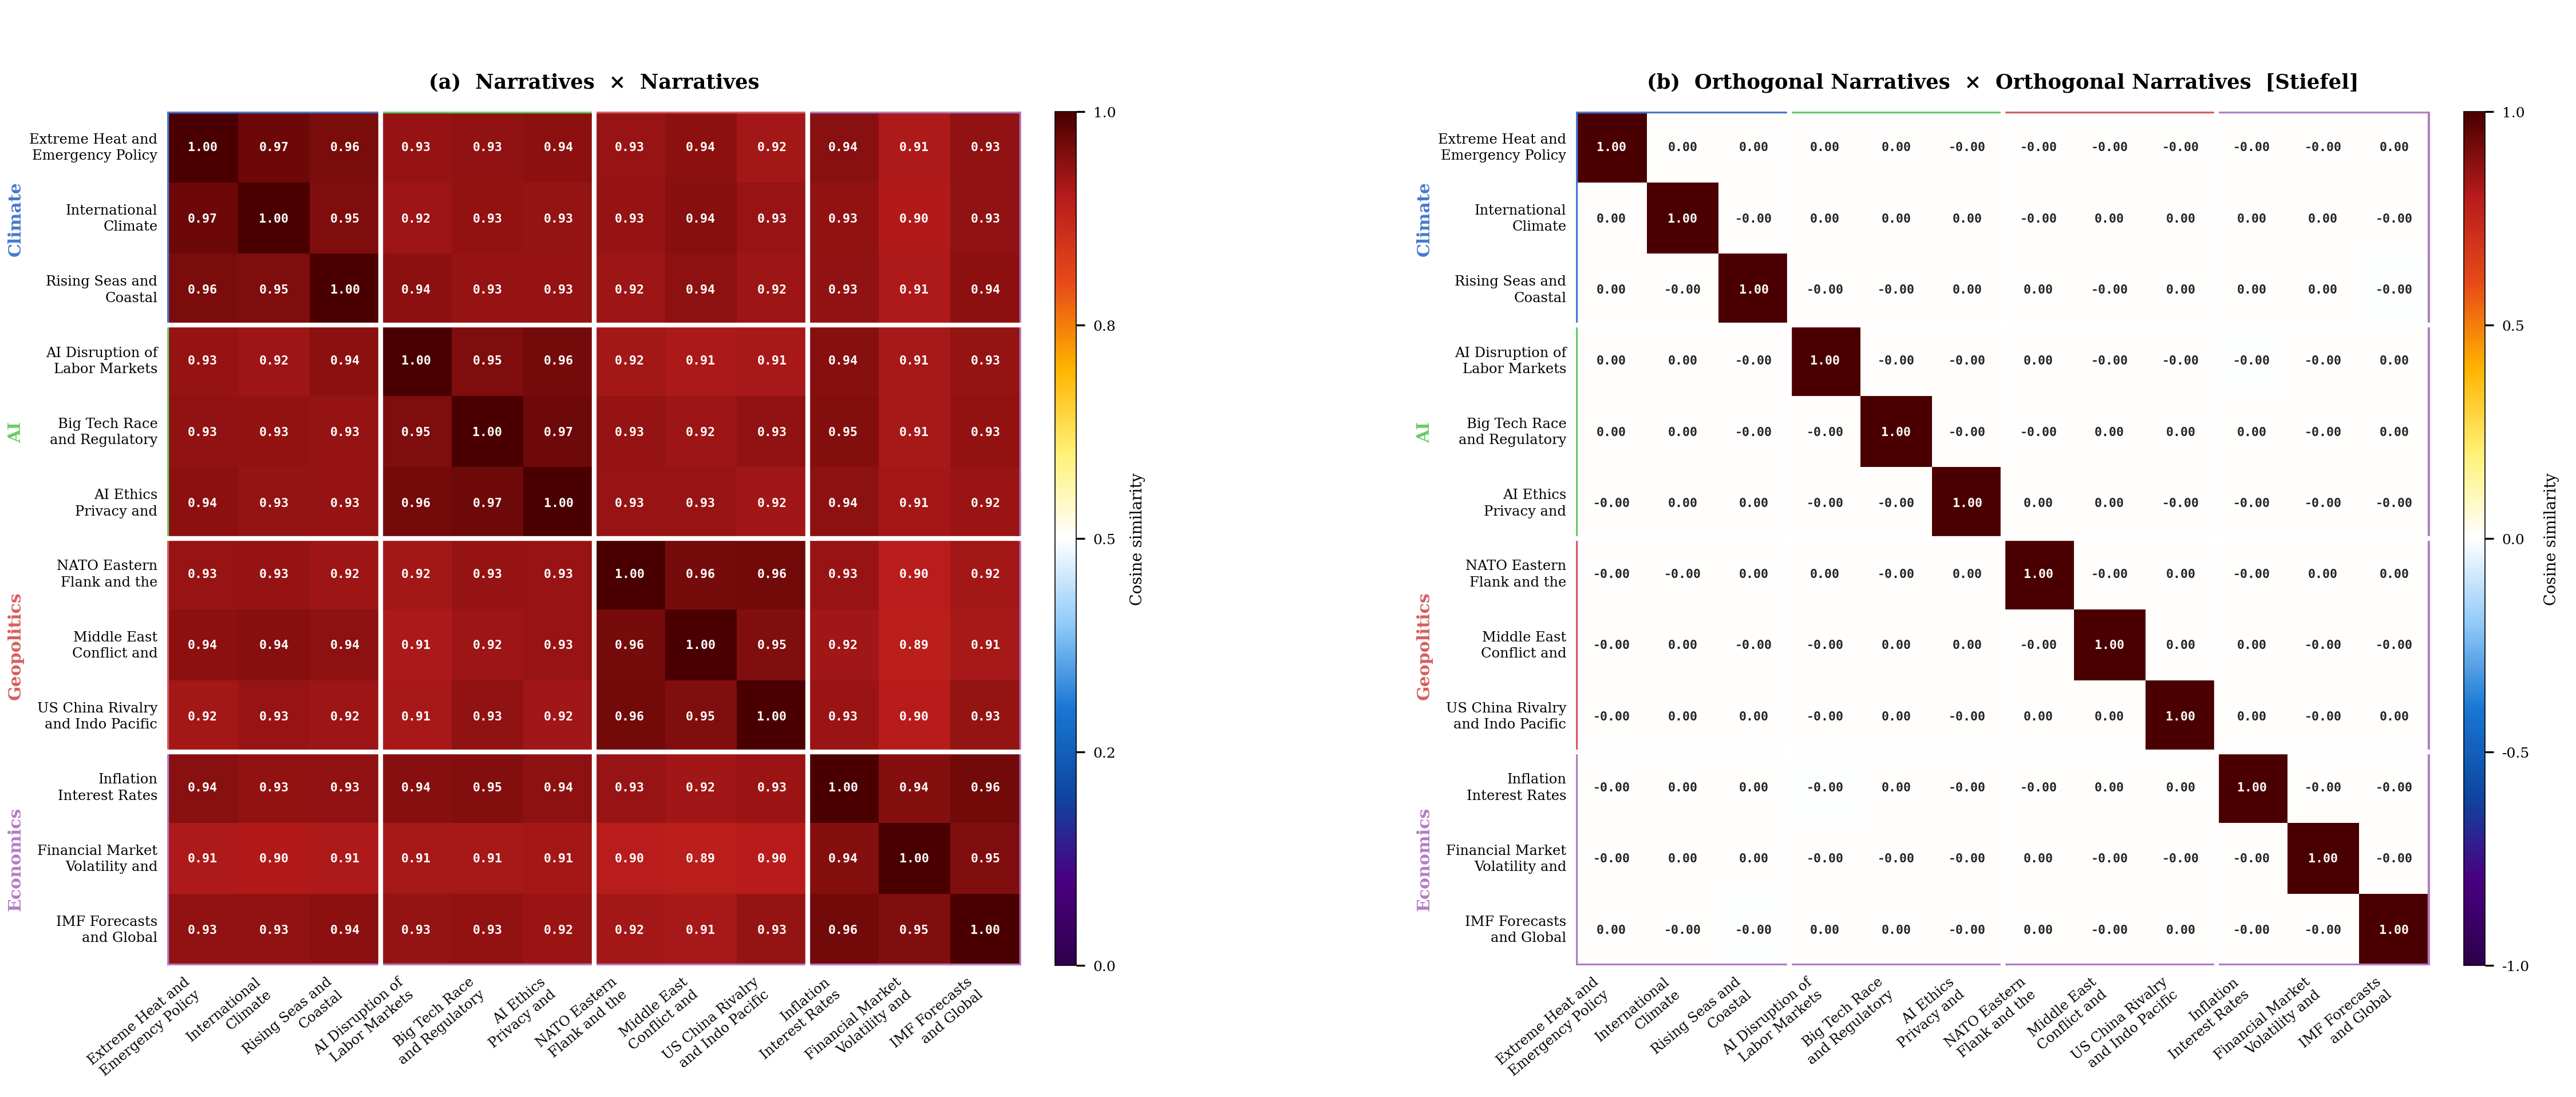
\includegraphics[width=\linewidth]{fig1_N_and_ON.png}
  \caption{Cosine similarity matrices of narrative embeddings before and after Stiefel orthogonalization. Panel~(a) shows the raw \textit{ModernBERT} embeddings, where diagonal blocks are systematically darker, reflecting stronger intra-chapter semantic 
cohesion. Panel~(b) shows the orthogonalized embeddings after Stiefel optimization, yielding zero pairwise cosine similarity across all narrative pairs thereby isolating the idiosyncratic semantic signal 
of each narrative.}
    \label{fig:cosine_matrix1}
\end{figure}



Panel (c) presents the cross-similarity between raw narratives and their Stiefel-optimized representatives. A clear diagonal structure emerges: each representative is more strongly correlated with its own source narrative than with any other, confirming that the optimization procedure preserves the idiosyncratic semantic content of each narrative while beginning to disentangle inter-narrative correlations.



Panel (d) exposes the limitations of the classical Gram-Schmidt orthogonalization. This procedure is well known to be sensitive to the ordering of input vectors: by construction, the first vector in the sequence is left entirely unchanged, while subsequent vectors are progressively deflated. As a result, the first representative, here that of \textit{"Extreme Heat and Emergency Policy Response"}, retains its original embedding and remains correlated with all other raw narratives. The pathological consequence is particularly striking: the representative of \textit{"Extreme Heat and Emergency Policy Response"} exhibits a higher cosine similarity with the raw narrative \textit{"Middle East Conflict and Humanitarian Crisis"}, for instance, than the representative of \textit{"Middle East Conflict and Humanitarian Crisis"} does with the very narrative it is supposed to represent. This severe distortion renders the Gram-Schmidt basis semantically uninterpretable as a set of narrative representatives, and underscores the superiority of the Stiefel-based approach for this task.





\begin{figure}[hbt!]
    \centering
    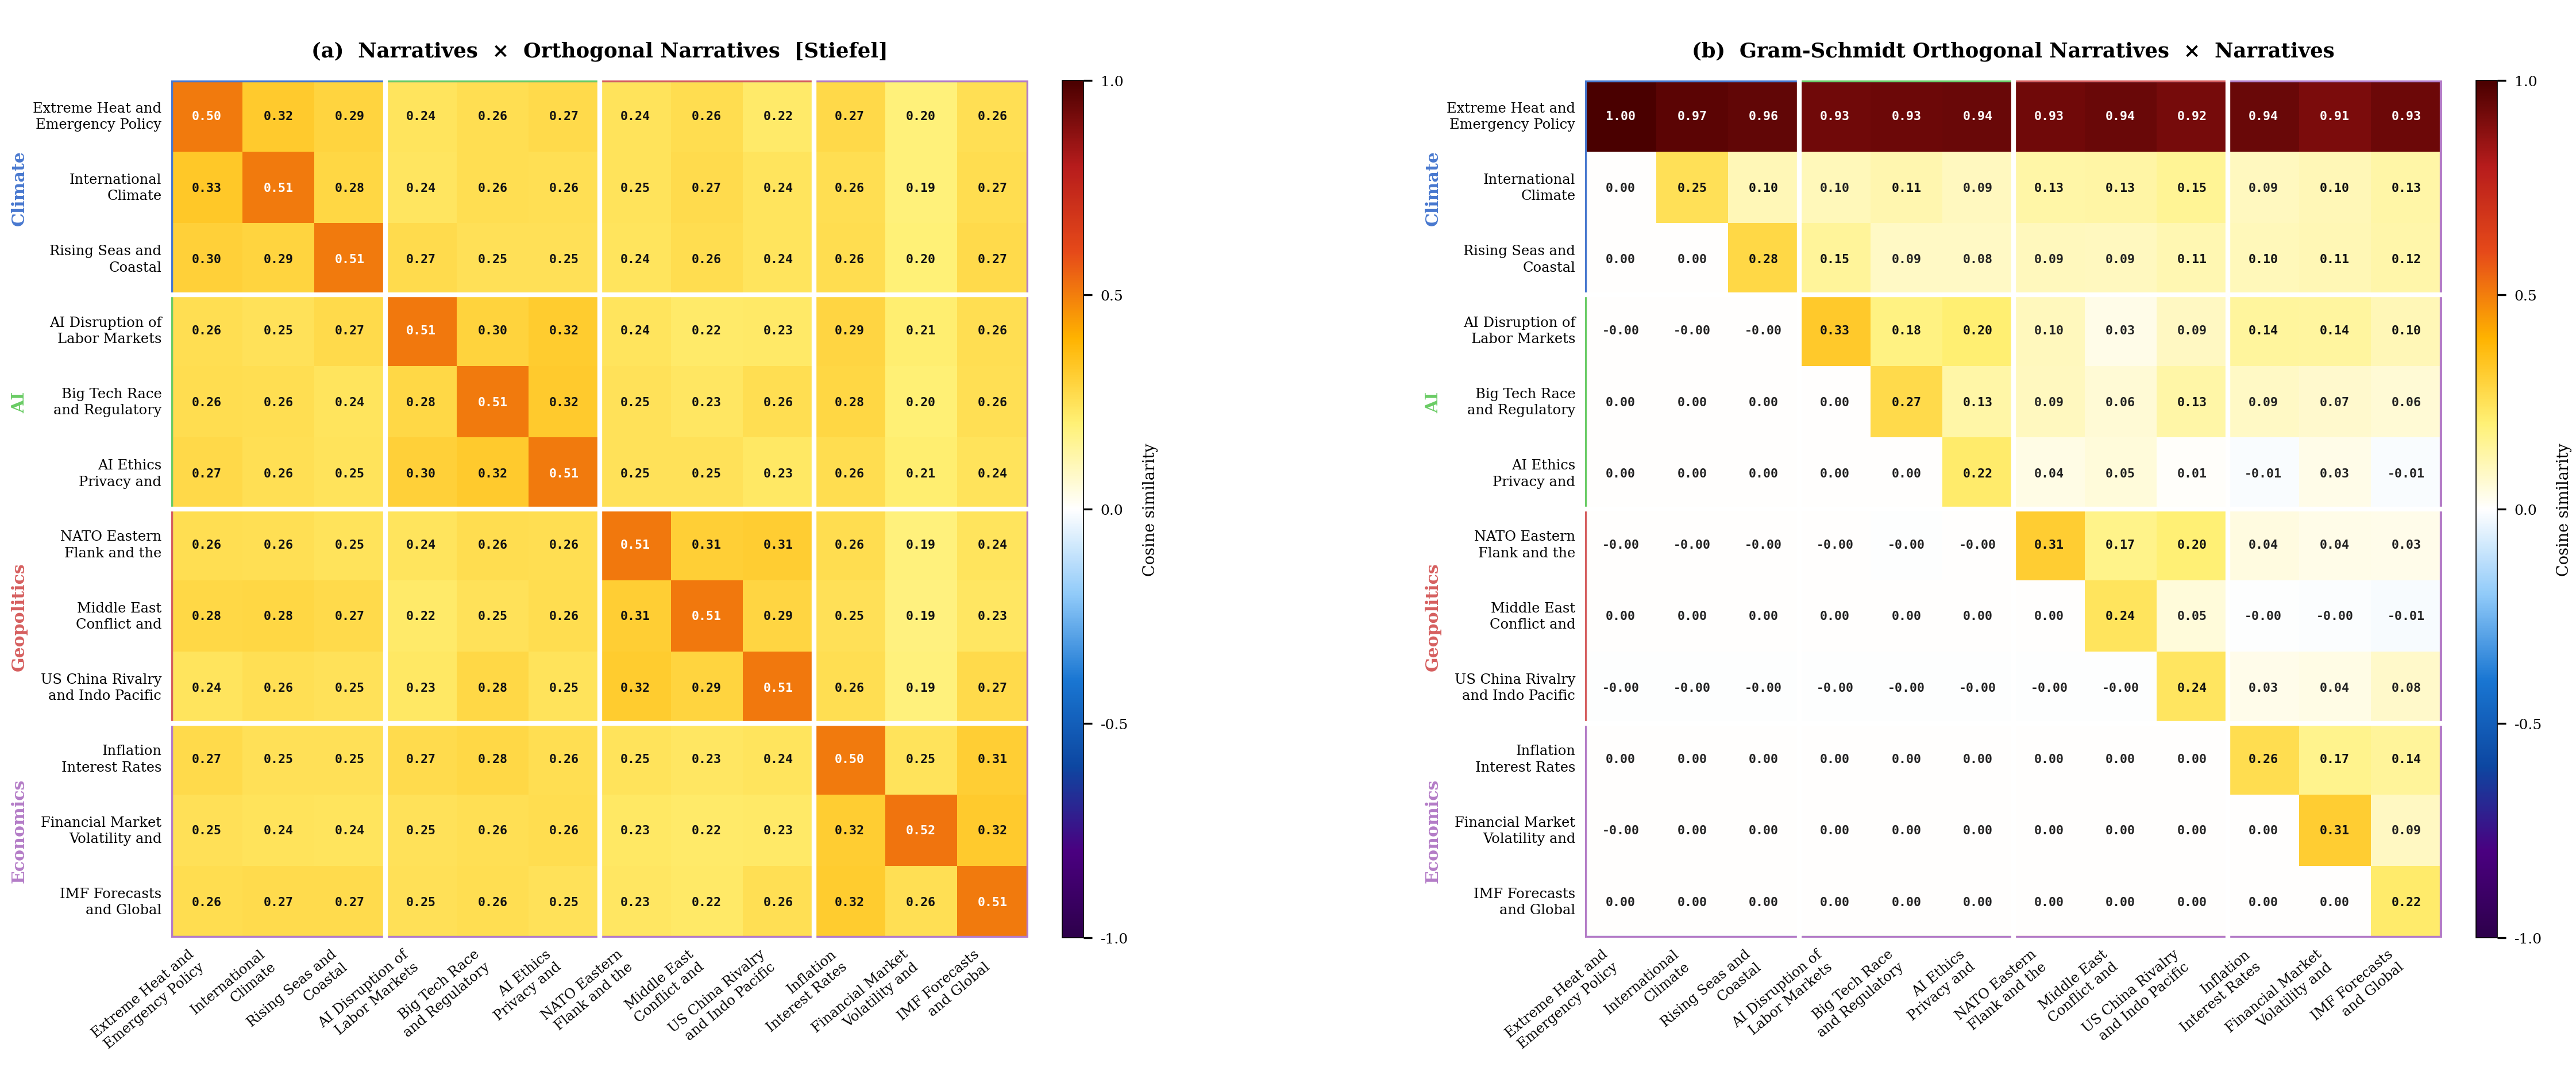
\includegraphics[width=\linewidth]{fig2_cross_and_GS.png}
\caption{Cross-similarity matrices between raw narrative embeddings and their orthogonalized representatives. Panel~(c) shows the Stiefel-optimized representatives, where a clear diagonal structure confirms that each representative retains the idiosyncratic semantic content of its source narrative. Panel~(d) shows the 
Gram-Schmidt representatives, revealing a severe order-dependent distortion: the first narrative is left unchanged and remains correlated with all others, to the point where its representative exhibits higher similarity with unrelated raw narratives than some narratives' own representatives do with themselves.}
    \label{fig:cosine_matrix2}
\end{figure}




%{\color{ForestGreen}
%Les tests sont de deux natures
%\begin{enumerate}
%    \item Il est plus difficile de faire la différence entre $V_1+\epsilon$ et $V_2+\epsilon$ (les $\epsilon$ étant corrélés) que entre $V_1$ et $V_2$.\\
%    En outre: c'est tout de même plus facile sur les $\hat p$ que sur les $\hat q$ (car dans le $\hat p$ il y a une partie TCL qui fait diminuer la variance due à $\epsilon$). 
%    \item Le contrefactuel sur Stiefel: Si on note 
%    $$\Delta^i(V_i) := \Esp((X^i)^\top V_i) - \Esp((X^{\neg i})^\top V_i)$$
%    l'écart entre la prévalence d'un narratif $i$ parmi les articles de son chapitre $i$ et celle parmi les articles des autres chapitres $\neg i$, on devrait avoir
%    $$\Delta^i(V_i) > \Delta^i(N_i).$$
%    C'est à dire que l'écart est plus grand lorsqu'on utilise les narratifs purs que lorsque ce n'est pas le cas.
%\end{enumerate}
%}











\bigskip 


\section{Experiments and Validation on a Dataset}
\label{sec:application}
\textcolor{ForestGreen}{\bf [CAL: expliquer qu'on utilise cette base car elle va permettre le contrefactuel + mettre en place le framework probabiliste pour les tests]}
\textcolor{ForestGreen}{\bf [CAL: alternatives à modernBERT]}
\JAMM{première recherche: https://chatgpt.com/share/69e58d30-f2c4-8329-aa4f-5682054e5775}


The objective of this empirical study is to validate the methodology introduced in the previous sections from two complementary perspectives. More precisely we will compare those two approaches: 
\begin{itemize}
    \item We use the embeddings that directly encodes the text representations of the studied collection of narratives. We denote them as $(N_i)_i$ and we will sometimes refer to them as \og raw narratives \fg. 
    \item We use the vectors obtained after applying the procedure described in \ref{sec:ortho:stiefel}. We denote them as $(V_i)_i$ and we will sometimes refer to them as \og pure narratives \fg or \og orthogonalized narratives \fg. 
\end{itemize}

We want to check that: 
\begin{itemize}
    \item That orthogonalized narratives effectively remove the biases highlighted in \ref{eq:generative:n};
    \item The orthogonalized representatives preserve the meaning;
    \item Tracking a document's similarity to an orthogonalized narrative is a more meaningful way to monitor the exposure to that specific narrative (compared to using the raw narratives)
\end{itemize}


To this end, we rely on the \emph{News Category Dataset}~\autocite{misra2022news}, whose manually assigned categories provide a natural counterfactual framework. 

\subsection{Dataset and Experimental Setup}
\label{sec:application:data}

\paragraph{Dataset.}
We use the \emph{News Category Dataset}~\autocite{misra2022news}, which contains approximately $210\,000$ headlines published by \emph{HuffPost} between 2012 and 2022. Since the archive becomes sparse after May 2018, we restrict the analysis to the 2012--2018 period, resulting in approximately $200\,000$ articles.

Among all available categories, we retain four sufficiently represented chapters:
\emph{Politics} ($32\,739$ articles), \emph{Entertainment} ($16\,058$),
\emph{Travel} ($9\,887$), and \emph{Parenting} ($8\,677$ articles). These four chapters naturally match the narrative groups introduced below and provide labeled subsets that can be exploited for validation.


\paragraph{Temporal resampling.}
The raw dataset is highly unbalanced over time, particularly for the Politics category during the 2016 presidential campaign. To avoid interpreting variations in publication volume as changes in narrative prevalence, we perform a temporal resampling that enforces a constant weekly number of articles while preserving the relative proportions across categories.Table~\ref{tab:resampled} reports the resulting distribution.

\TODO{Ici, il y a sans doute un commentaire à faire sur les catégories (les seules ok à mon avis c'est entertainment et politics) - ce qui n'empêche pas d'utiliser les autres si on moyenne sur toute la période}

\begin{table}[hbt!]
\begin{threeparttable}
\caption{Number of articles per category and year after resampling.}
\label{tab:resampled}
\begin{tabular}{lrrrr}
\toprule
\headrow Year & Entertainment & Parenting & Politics & Travel \\
\midrule
2012 &   792 & 4{,}087 &         0 & 4{,}221 \\
2013 & 1{,}154 & 4{,}710 &         0 & 3{,}786 \\
2014 & 2{,}445 & 1{,}403 & 3{,}684 & 2{,}079 \\
2015 & 3{,}614 &         0 & 5{,}351 &    705 \\
2016 & 2{,}478 &         0 & 6{,}885 &    311 \\
2017 & 2{,}194 &         0 & 7{,}273 &    178 \\
2018 & 1{,}375 &         0 & 2{,}450 &     60 \\
\bottomrule
\end{tabular}
\end{threeparttable}
\end{table}


\paragraph{Embeddings.}
Both news headlines and narrative descriptions are embedded in the same $768$-dimensional semantic space using \emph{ModernBERT}~\autocite{warner2024modernbert}. Narrative descriptions were generated with the assistance of a large language model to ensure a homogeneous writing style.

\subsection{Narratives}

For each of the four chapters, we manually define three representative narratives intended to capture the main social, political, and cultural themes that characterize the corresponding articles over the 2012--2018 period. The complete list of the twelve narratives is provided in \ref{app:narratives}. A selection is shown below.

\begin{table}[hbt!]
\begin{threeparttable}
\caption{Narratives used in the analysis (selection).}
\label{tab:narratives_short}
\begin{tabular}{llp{6cm}}
\toprule
\headrow Chapter & Narrative & Description \\
\midrule
Politics
  & Trump as Disruptor and Institutional Stress
  & Donald Trump rises to power by channeling distrust toward political elites,
    media institutions, and bureaucratic authority, presenting himself as a
    disruptive outsider challenging democratic norms. \\
\addlinespace
Entertainment
  & Entertainment as Political Resistance
  & Film, television, comedy, and celebrity culture become arenas of political
    contestation blending entertainment with explicit political messaging. \\
\addlinespace
Parenting
  & The Overwhelmed Modern Parent
  & Parenthood is portrayed as emotionally intense and structurally unsupported,
    with parents struggling to balance careers, childcare costs, and social
    expectations. \\
\addlinespace
Travel
  & Experiential and Transformational Travel
  & Travel is framed as a path to personal growth and cultural immersion through
    encounters with landscapes, heritage sites, and local communities. \\
\bottomrule
\end{tabular}
\end{threeparttable}
\end{table}

The raw narrative embeddings are then orthogonalized using the Stiefel optimization procedure described in Section~\ref{sec:ortho}, producing the corresponding \textit{collection of pure narratives} $(V_i)_i$.

\subsection{First qualitative results}
\label{sec:application:qualitative}

We first perform a qualitative comparison between the prevalence estimators obtained using the raw narrative vectors $N_i$ and their orthogonalized representatives $V_i$.

To facilitate visual interpretation, we restrict this analysis to the Politics and Entertainment chapters over the 2014--2018 period, where both categories contain a sufficiently balanced number of observations. The displayed curves correspond to an exponential moving average of the estimator $\hat p_i(t)$ introduced in Section~\ref{sec:model}.



\begin{figure}[h!]
    \centering
    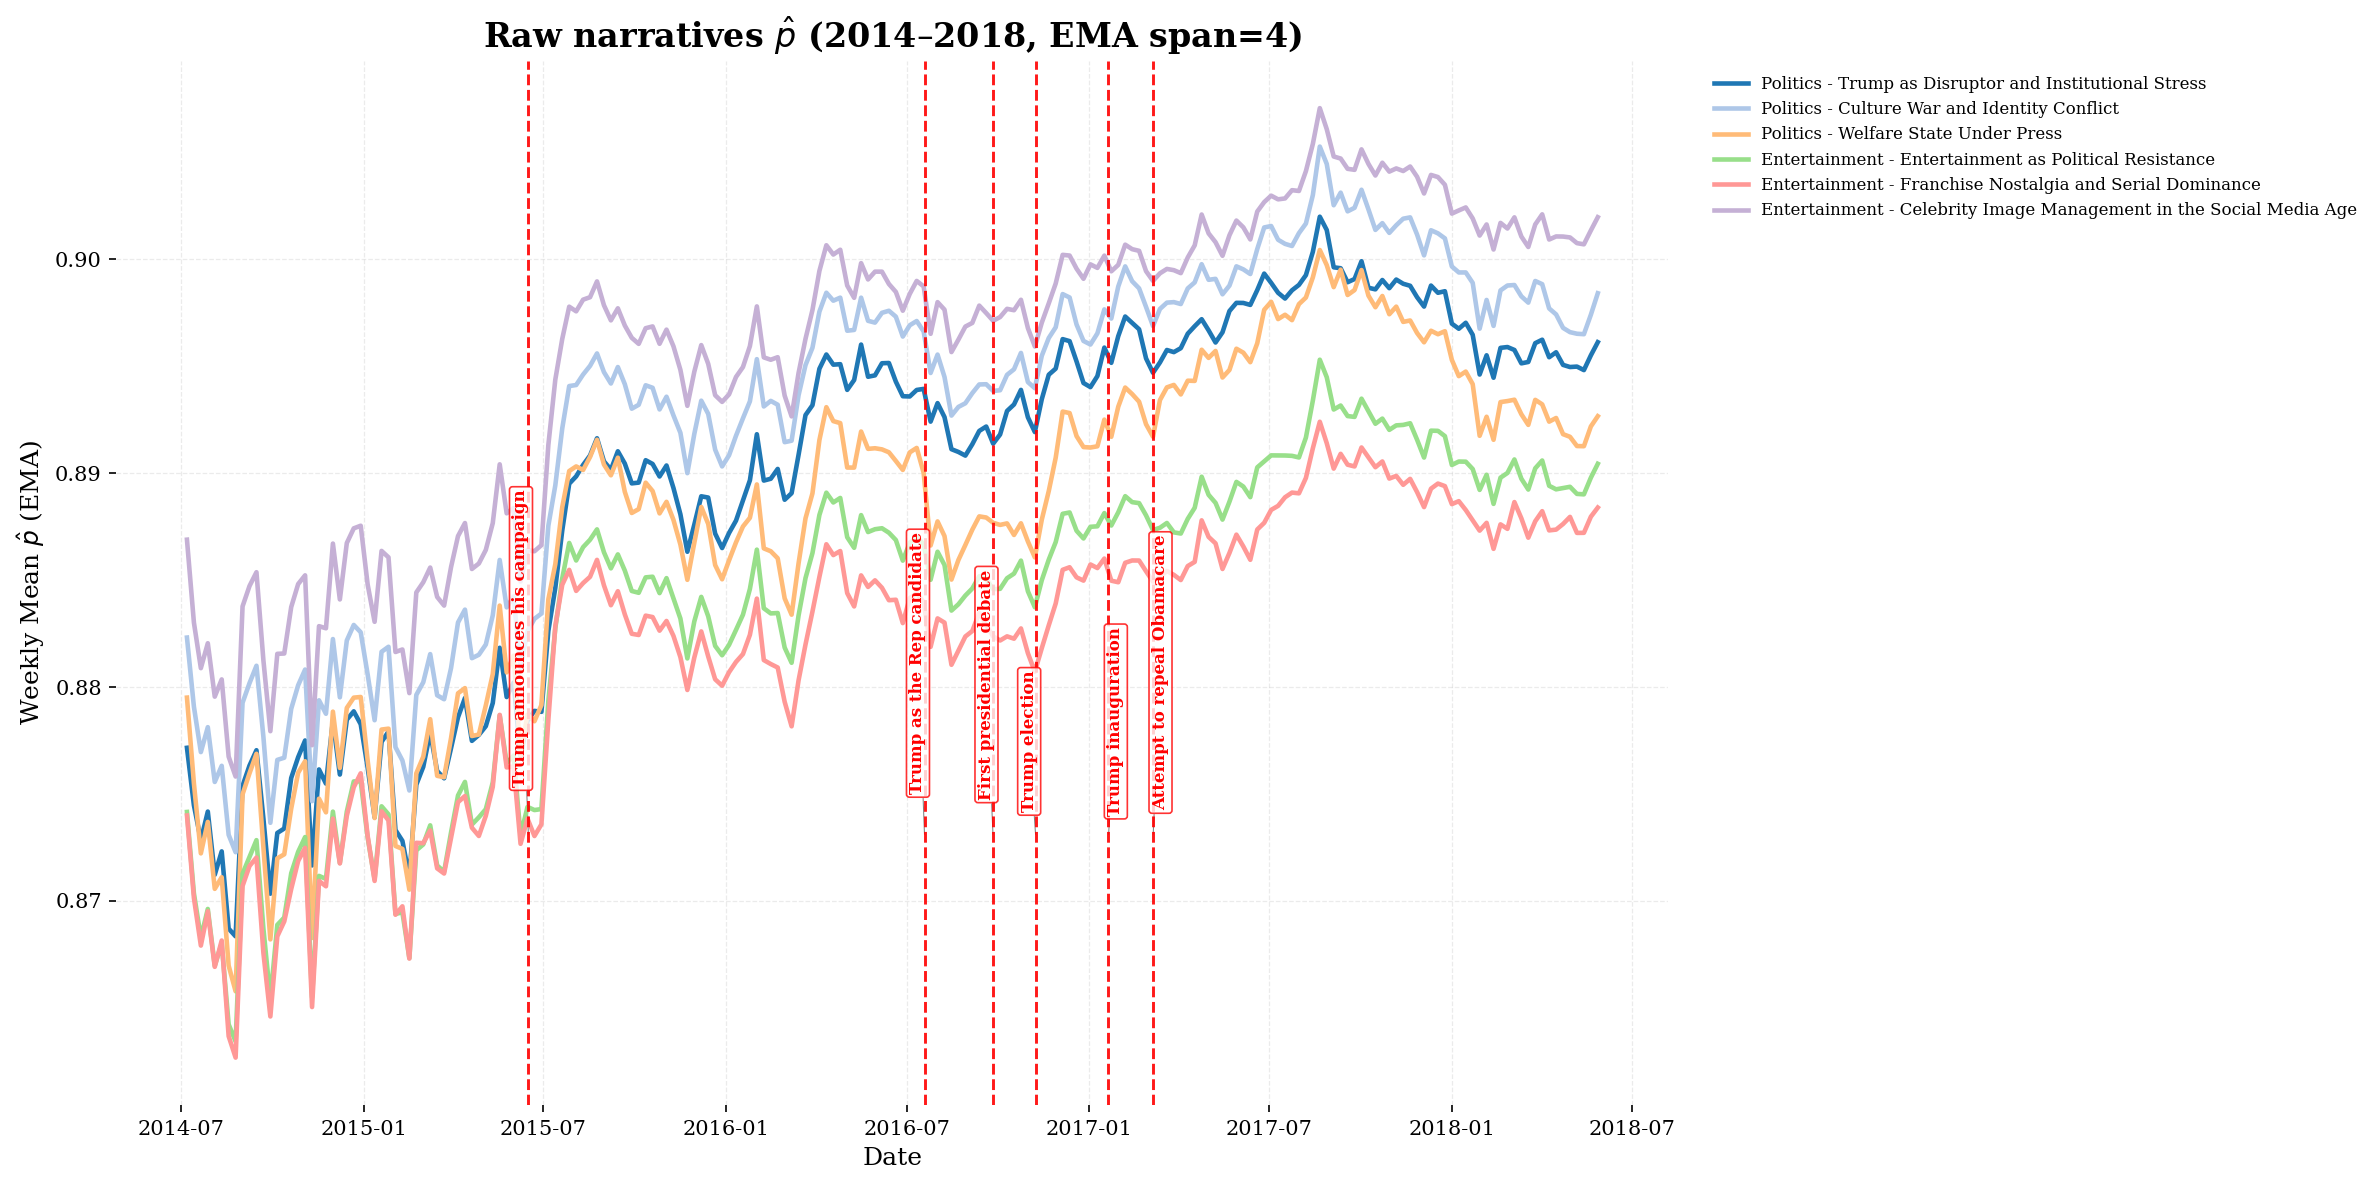
\includegraphics[width=0.7\textwidth]{EMA15oct.png}
    \vspace{0.3cm}

    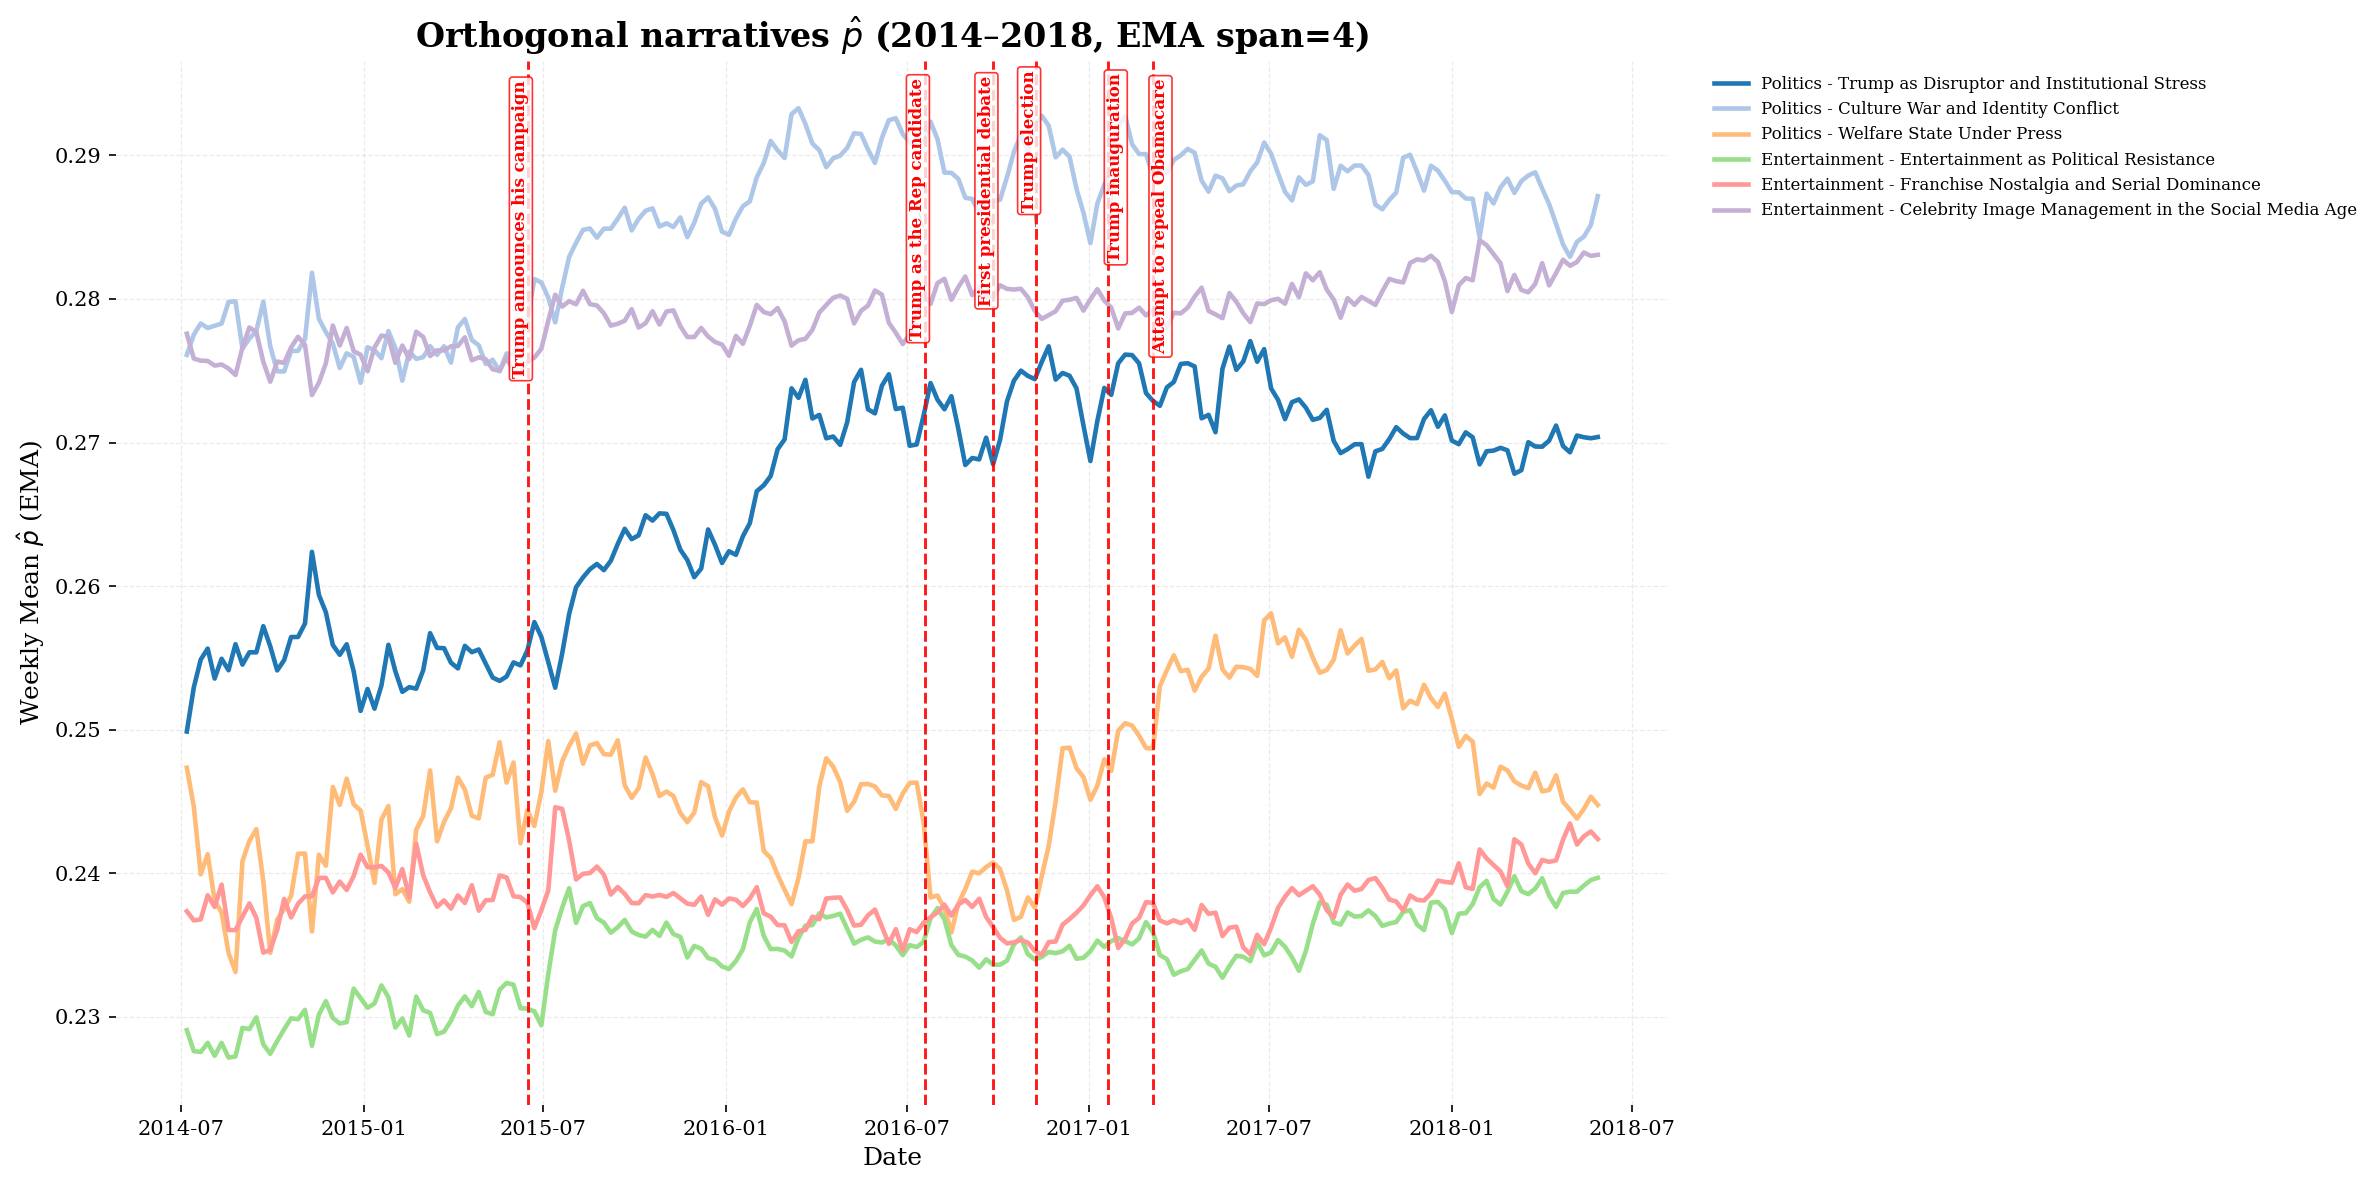
\includegraphics[width=0.7\textwidth]{EMAorth15oct.png}
    \caption{Time series of EMA weekly means of cosine similarities for raw and orthogonal narratives.}
    \label{fig:ema_comparison}
\end{figure}

The contrast between the two approaches is immediate. Under the raw narrative vectors, the prevalence series evolve almost perfectly synchronously, illustrating the leakage phenomenon anticipated in Section~\ref{sec:model}: when the prevalence of an unrelated but semantically connected narrative rises, the naive prevalence indicator computed on raw narratives increases mechanically along with it. Pure narratives, by contrast, produce clearly differentiated temporal trajectories, with each of them now exhibiting its own distinctive dynamics.

The clearest visual illustration of this contrast occurs between January 2017 and January 2018, when a pronounced bump appears in the raw prevalence series of virtually every narrative. Under the purified representation, this bump is observed almost exclusively in the \emph{Welfare State Under Pressure} narrative, the only one for which it plausibly reflects genuine content rather than a shift shared indiscriminately across the corpus. This single episode captures the practical interest of orthogonalization: without it, an apparent surge in any given narrative could just as easily be an artifact of another, unrelated narrative's rise. This pattern is consistent with the historical record, as the early months of the Trump administration were marked by sustained legislative pressure on the social safety, most notably through repeated attempts to repeal the Affordable Care Act (Obamacare).

The observed behavior is also consistent with the historical context used to design the narratives. The political narratives were deliberately chosen to capture the rise of Donald Trump's presidential campaign and its associated political themes. Accordingly, the prevalence of the narratives \emph{Trump as Disruptor and Institutional Stress} and \emph{Culture War and Identity Conflict} increases steadily throughout the campaign and reaches its highest levels around the 2016 election. This evolution is qualitatively consistent with the growing importance of these themes in the political debate.

Conversely, the Entertainment narratives were intentionally designed to represent long-term structural trends rather than isolated historical events. Their estimated prevalence therefore remains comparatively stable over time, exhibiting only moderate fluctuations. The resulting time series are thus coherent with the expected temporal behavior of the corresponding narratives.



\subsection{Co-variation, semantic specificity and rupture tests}
\JAMM{TO DO: changer le titre}
\label{sec:application:quantitative}

We next evaluate the proposed methodology through three complementary quantitative experiments.

\paragraph{Reduction of artificially high co-variation}
We first observe qualitatively that the prevalence curves within the political and Entertainment subsets of narratives evolve almost synchronously. We now turn to quantifying this phenomenon across the full set of narratives under study.

We use the metric introduced in Section~\ref{sec:model}:
\[
M_{ij}(t) := \mathbb{E}\bigl[(X_n^\top W_i)(X_n^\top W_j)\mid\mathcal{F}_t\bigr], \qquad n\in\mathcal{C}_t.
\]
As discussed there, for a collection of raw, non-orthogonalized narratives, two distinct effects artificially inflate this covariation: signal leakage and the correlation induced by the noise term. We therefore assess whether orthogonalization produces a sizable reduction in covariation. Time is discretized weekly: for each pair $(i,j)$ we compute $M_{ij}(t)$ and average it over the entire study period.

\begin{table}[ht]
\centering
\begin{tabular}{lcc}
\toprule
 & N (raw) & V (purified) \\
\midrule
mean & 74.018 & 6.486 \\
std & 0.646 & 0.737 \\
median & 73.985 & 6.421 \\
min & 72.775 & 5.209 \\
max & 75.546 & 8.343 \\
\bottomrule
\end{tabular}
\caption{Descriptive statistics of pairwise narrative covariation $M_{ij}(t)$ ($\times 10^{-7}$), before (N) and after (V) orthogonalization.}
\label{tab:covariation_stats}
\end{table}

The empirical results strongly support this prediction: as reported in Table~\ref{tab:covariation_stats}, pairwise covariation scores computed from the raw narrative vectors are, on average, approximately one order of magnitude larger than those obtained after orthogonalization.

\paragraph{Semantic specificity.}

The second validation exercise aims to verify that purified representatives preserve the semantic meaning of the original narratives.

The labeled structure of the News Category Dataset naturally provides a counterfactual framework: since every narrative belongs to one of four chapters, we compare its average cosine similarity within its own chapter to its average similarity outside that chapter.

For the orthogonalized representatives, we define

\[
\Delta^{i,k}(V_{i,k})
=
\mathbb{E}
\!\left[
(X^{i})^\top V_{i,k}
\right]
-
\mathbb{E}
\!\left[
(X^{\neg i})^\top V_{i,k}
\right],
\]

where $X^{i}$ denotes articles belonging to chapter $i$, while $X^{\neg i}$ denotes all remaining articles.

The analogous quantity is computed for the original narrative vectors,

\[
\Delta^{i,k}(N_{i,k})
=
\mathbb{E}
\!\left[
(X^{i})^\top N_{i,k}
\right]
-
\mathbb{E}
\!\left[
(X^{\neg i})^\top N_{i,k}
\right].
\]

A meaningful narrative should be more strongly represented within its own chapter than outside it, implying

\[
\Delta^{i,k}(N_{i,k})>0,
\qquad
\Delta^{i,k}(V_{i,k})>0.
\]

More importantly, if orthogonalization successfully removes semantic information shared with other chapters while preserving each narrative's intended meaning, we expect

\[
\Delta^{i,k}(V_{i,k})
>
\Delta^{i,k}(N_{i,k}).
\]



\begin{table}[htbp]
\centering
\caption{Sensitivity analysis: 1000 bootstrap draws, 100\% of articles, 95\% CI for $\Delta^{i}(V_{i})$,$\Delta^{i}(N_{i})$, and $\Delta_{\text{gain}} = \Delta^i(V_i) - \Delta^i(N_i)$}
\label{tab:sensitivity_analysis}
\small
\setlength{\tabcolsep}{4pt}
\renewcommand{\arraystretch}{1.15}
\resizebox{\textwidth}{!}{%
\begin{tabular}{llccc}
\toprule
\textbf{Chapter} &
\textbf{Narrative} &
$\boldsymbol{\Delta^i(N_i)}$ &
$\boldsymbol{\Delta^i(V_i)}$ &
$\boldsymbol{\Delta_{\text{gain}}}$ \\
\midrule
Politics &
Trump as disruptor and institutional stress &
$0.0019$ [0.0015, 0.0023] &
$0.0377$ [0.0374, 0.0381] &
$0.0358$ [0.0353, 0.0363] \\

Politics &
Culture war and identity conflict &
$-0.0002$ [-0.0006, 0.0003] &
$0.0312$ [0.0309, 0.0316] &
$0.0314$ [0.0309, 0.0319] \\

Politics &
Welfare state under press &
$-0.0053$ [-0.0058, -0.0048] &
$0.0084$ [0.0078, 0.0090] &
$0.0137$ [0.0134, 0.0141] \\

Entertainment &
Entertainment as political resistance &
$-0.0145$ [-0.0151, -0.0139] &
$0.0062$ [0.0058, 0.0066] &
$0.0207$ [0.0203, 0.0210] \\

Entertainment &
Franchise nostalgia and serial dominance &
$-0.0107$ [-0.0112, -0.0101] &
$0.0207$ [0.0202, 0.0211] &
$0.0313$ [0.0309, 0.0318] \\

Entertainment &
Celebrity image management in the social media... &
$-0.0153$ [-0.0159, -0.0148] &
$0.0054$ [0.0050, 0.0058] &
$0.0207$ [0.0202, 0.0212] \\

Parenting &
The overwhelmed modern parent &
$0.0253$ [0.0249, 0.0256] &
$0.0118$ [0.0114, 0.0123] &
$-0.0134$ [-0.0139, -0.0129] \\

Parenting &
Intensive and expert guided parenting &
$0.0287$ [0.0283, 0.0291] &
$0.0302$ [0.0297, 0.0308] &
$0.0015$ [0.0010, 0.0020] \\

Parenting &
Raising children in a politicized society &
$0.0244$ [0.0240, 0.0248] &
$0.0174$ [0.0171, 0.0178] &
$-0.0070$ [-0.0073, -0.0066] \\

Travel &
Experiential and transformational travel &
$0.0251$ [0.0246, 0.0257] &
$0.0298$ [0.0293, 0.0304] &
$0.0047$ [0.0042, 0.0052] \\

Travel &
Travel optimization and consumer strategy &
$0.0279$ [0.0274, 0.0285] &
$0.0415$ [0.0410, 0.0420] &
$0.0135$ [0.0130, 0.0141] \\

Travel &
Aesthetic and instagrammable destinations &
$0.0297$ [0.0293, 0.0303] &
$0.0452$ [0.0446, 0.0458] &
$0.0155$ [0.0150, 0.0160] \\
\bottomrule
\end{tabular}%
}
\end{table}

The results are satisfactory: every chapter exhibits $\Delta^i(V_i) > 0$, whereas the Entertainment chapter and two narratives of Politics chapter have $\Delta^i(N_i) < 0$. Regarding $\Delta_{\text{gain}}$, it is positive for three chapters out of four.

\paragraph{Narrative specificity of detected ruptures}

We now quantify the qualitative observation made above: ruptures detected on raw narrative representations tend to be shared across many, otherwise unrelated, narratives, whereas ruptures detected on purified representations are largely specific to a single narrative.

For a narrative representation $M \in \{N_i, V_i\}$ and each candidate date $t$, let $\mathcal{B}_t$ and $\mathcal{A}_t$ denote the sets of articles published, respectively, in the 90-day window preceding and following $t$. Writing $Q_n(M) = X_n^\top M$ for the projected score of article $n$, we test, at every candidate date $t$,
\[
H_0 : \mathbb{E}\bigl[Q_n(M) \mid n \in \mathcal{B}_t\bigr] = \mathbb{E}\bigl[Q_n(M) \mid n \in \mathcal{A}_t\bigr],
\]
using a two-sided Welch $t$-test, which does not require equal variances across the two windows. Because this test is repeated over hundreds of candidate dates, the resulting $p$-values are corrected for multiple testing using the Benjamini-Hochberg FDR procedure; consecutive significant dates are then grouped into a single detected rupture. This procedure is applied separately to the raw ($N$) and purified ($V$) representations of every narrative in our collection.

Results are reported in Figures~\ref{fig:my_label} Three observations stand out.

First, the number of detected ruptures is systematically higher under $N$ than under $V$: averaged across narratives, $27.1$ ruptures are detected under $N$, against $16.5$ under $V$, and this ordering holds narrative by narrative without exception.

Second, pairwise overlap between the sets of rupture dates detected across different narratives is markedly higher under $N$ than under $V$, as measured by the Jaccard index\footnote{Jaccard index: $J(A,B) = \dfrac{|A \cap B|}{|A \cup B|}$.}: the average pairwise Jaccard index is $0.74$ under $N$, compared to only $0.25$ under $V$. Taken together, these two findings confirm that raw representations tend to co-detect the same, corpus-wide ruptures, consistent with the leakage phenomenon described in Section~\ref{sec:model:generative_model}, whereas purified representations isolate ruptures that are substantially more specific to each individual narrative.

Third, this is directly illustrated by the July 2017 bump discussed in our qualitative analysis: under $N$, it is detected as a significant rupture for every narrative in the collection, while under $V$ it is detected almost exclusively for the \emph{Welfare State Under Pressure} narrative, the only one for which it plausibly reflects genuine, narrative-specific content (as the period corresponds to Trump's first semester as President with notably repeated attempt to repeal the Obamacare) rather than a shift shared indiscriminately across the corpus.



\begin{figure}[h!]
    \centering
    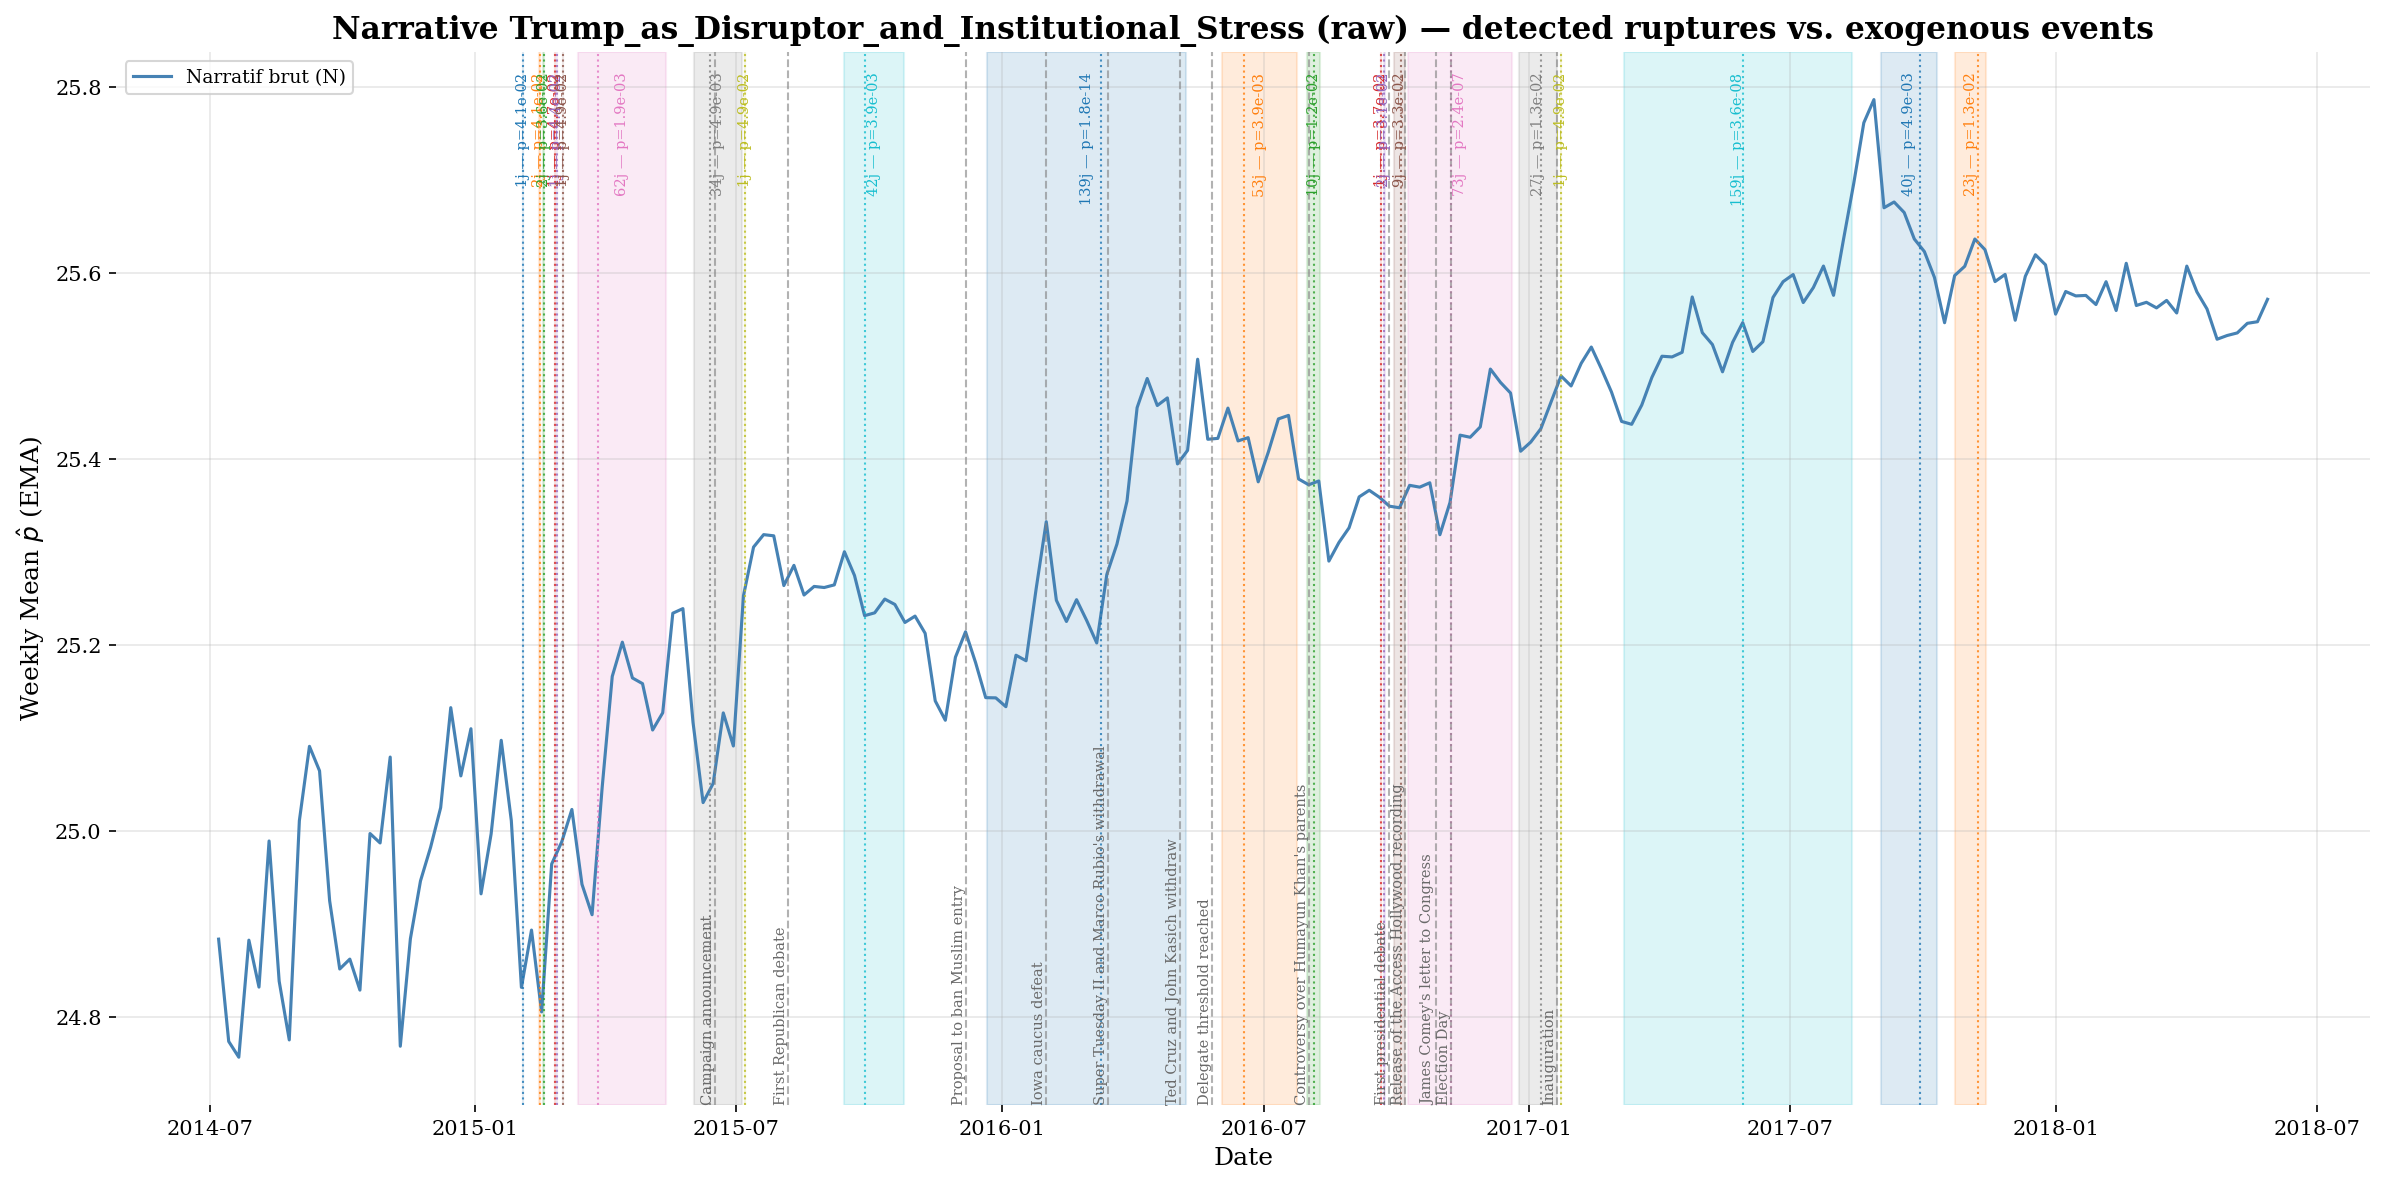
\includegraphics[width=0.7\textwidth]{ruptureTrump.png}
    \vspace{0.3cm}

    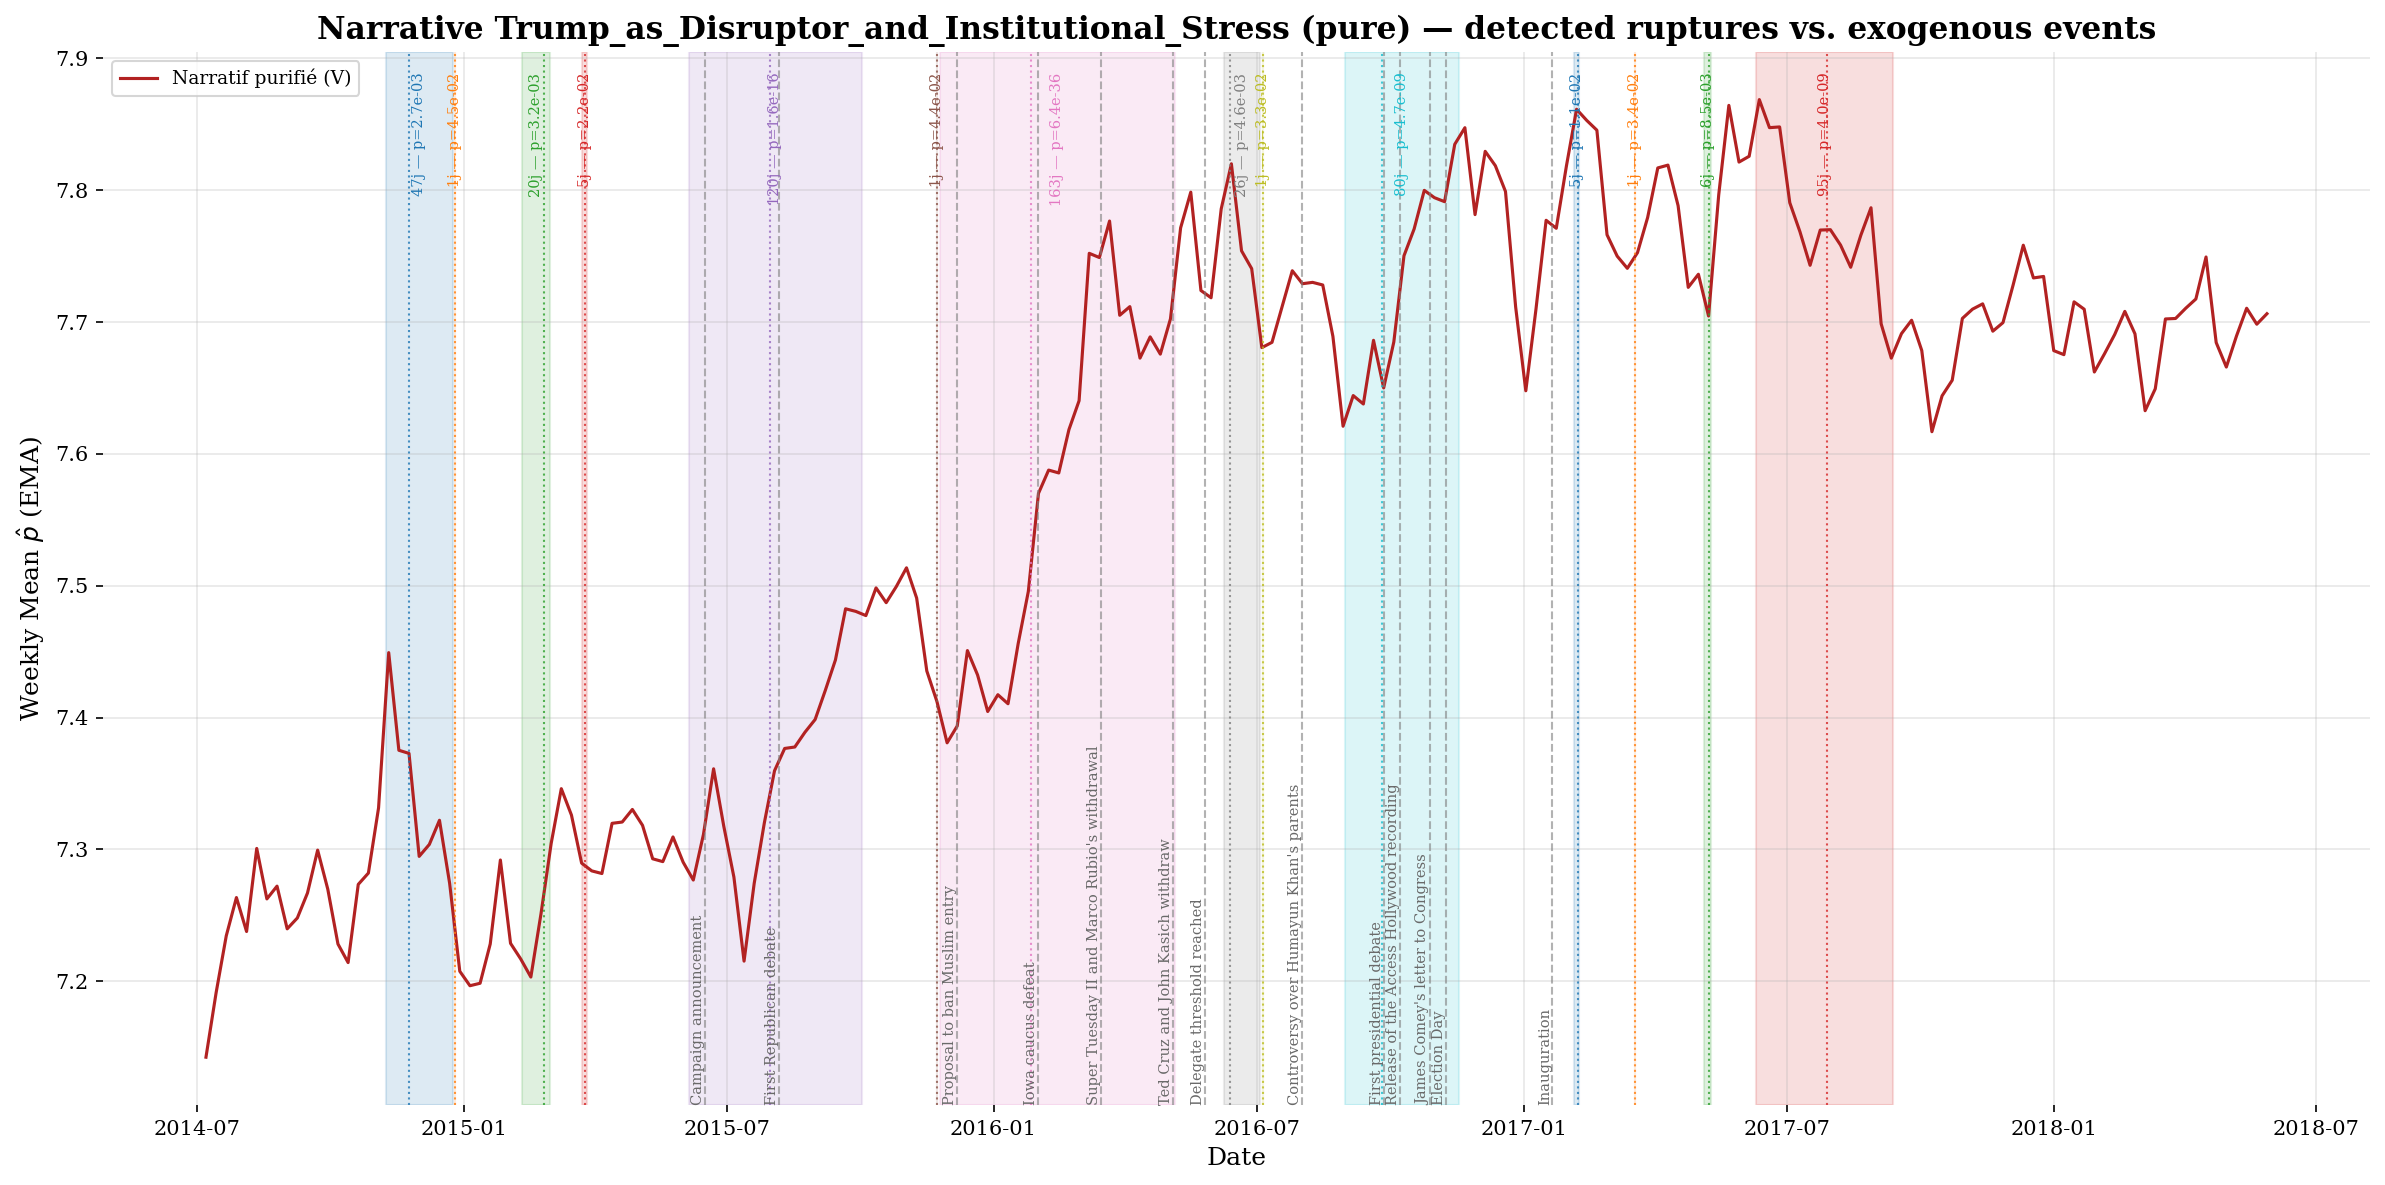
\includegraphics[width=0.7\textwidth]{ruptureTrumporth.png}
    \caption{Time series of EMA weekly means of cosine similarities for raw and orthogonal Trump narrative, with detected ruptures as well as a set of exogenous events related to Trump's campaign.} %\href{https://www.cjr.org/special_report/trump-coverage-election-clinton.php}{Trump's campaign}
    \label{fig:rupture_comparison}
\end{figure}












\bigskip




% -------------------------------------------------------
\section{Conclusion}
\label{sec:conclusion}
% -------------------------------------------------------

We have introduced a rigorous algebraic methodology for monitoring the relative
prevalence of competing narratives in a time-evolving text corpus.
The key insight is that standard cosine similarity between article embeddings
and raw narrative vectors suffers from a structural correlation bias induced
by shared semantic content, which we characterize formally through a linear
generative model.

Our remedy---a global orthogonalization on the Stiefel manifold---eliminates
this shared component while preserving each narrative's idiosyncratic direction,
yielding an unbiased, non-parametric, and interpretable prevalence estimator.
Validation on a large labeled news corpus confirms that the estimator
faithfully recovers known historical dynamics, whereas the naive approach fails.

\paragraph{Perspectives.}
The natural extension of this work is the application of the estimator to
large-scale financial news corpora, opening the way to a direct quantitative
model of narrative competition and its influence on the formation of
economic expectations---a question at the intersection of computational linguistics
and market microstructure.

\paragraph{Acknowledgments}
We are grateful for the technical assistance of \TODO{add acknowledgments}.

\paragraph{Funding Statement}
\TODO{Insert funding statement or `None'.}

\paragraph{Competing Interests}
None.

\paragraph{Data Availability Statement}
The News Category Dataset is publicly available~\autocite{misra2022news}. Replication code can be found at \TODO{insert repository URL}.

\paragraph{Ethical Standards}
The research meets all ethical guidelines, including adherence to the legal requirements of the study country.

\paragraph{Author Contributions}
Conceptualization: J.A., M.M., C.-A.L. Methodology: J.A., M.M., C.-A.L. Data curation: J.A., M.M. Data visualisation: J.A., M.M. Writing original draft: J.A., M.M., C.-A.L. All authors approved the final submitted draft.

\printendnotes

\TODO{Est-ce que c'est léger en termes de références ?}

\printbibliography

\appendix

\section{Complete List of Narratives as an Illustration}
\label{app:narratives_illustration}

\begin{longtable}{p{2cm}p{4cm}p{7cm}}
\caption{All narratives used in the analysis.}
\label{tab:narratives}\\
\toprule
\textbf{Chapter} & \textbf{Narrative} & \textbf{Description} \\
\midrule
\endfirsthead

\multicolumn{3}{c}{\tablename\ \thetable{} -- \textit{Continued from previous page}} \\
\toprule
\textbf{Chapter} & \textbf{Narrative} & \textbf{Description} \\
\midrule
\endhead

\midrule
\multicolumn{3}{r}{\textit{Continued on next page}} \\
\endfoot

\bottomrule
\endlastfoot

Climate
  & Extreme Heat and Emergency Policy Response
  & Record-breaking temperatures across southern Europe this summer triggered
    unprecedented heatwaves, forcing governments to activate emergency climate plans
    and accelerate the transition toward renewable energy sources in order to
    meaningfully reduce carbon emissions and limit further global warming. \\
Climate
  & International Climate Commitments Under Pressure
  & As climate-related disasters multiply worldwide, the United Nations urgently calls
    for stronger adherence to the Paris Agreement, emphasizing that industrialized
    nations must deliver substantial and verifiable reductions in greenhouse gas
    emissions before irreversible climate tipping points are reached. \\
Climate
  & Rising Seas and Coastal Vulnerability
  & The accelerating melting of Arctic glaciers, driven by sustained global warming,
    is causing a gradual but measurable rise in sea levels that threatens tens of
    millions of people living in low-lying coastal zones, according to a major
    scientific report released this week. \\
\addlinespace
Artificial Intelligence
  & AI Disruption of Labor Markets
  & The rapid rise of generative artificial intelligence models is profoundly reshaping
    global labor markets, prompting technology companies to invest billions of dollars
    in autonomous systems capable of gradually replacing skilled workers across a wide
    range of industries and professional sectors. \\
Artificial Intelligence
  & Big Tech Race and Regulatory Pushback
  & Silicon Valley's leading technology firms are intensifying their competition in
    artificial intelligence by unveiling increasingly powerful language models, while
    European regulators work to constrain these developments through strict legislative
    frameworks designed to protect citizens' fundamental rights and digital freedoms. \\
Artificial Intelligence
  & AI Ethics, Privacy, and Public Sector Governance
  & Recent breakthroughs in artificial intelligence are raising critical ethical
    concerns around personal data privacy and cybersecurity, prompting several national
    governments to establish dedicated regulatory frameworks governing the deployment
    of these technologies within public institutions and essential services. \\
\addlinespace
Geopolitics
  & NATO Eastern Flank and the Russia--Ukraine War
  & The ongoing military conflict between Russia and Ukraine continues to destabilize
    the European geopolitical order, compelling NATO allies to reinforce their eastern
    flank with additional troops and to significantly increase national defense budgets
    in response to sustained and escalating Russian aggression. \\
Geopolitics
  & Middle East Conflict and Humanitarian Crisis
  & The armed conflict in the Middle East has triggered a humanitarian catastrophe of
    alarming proportions, prompting urgent international calls for an immediate
    ceasefire and the rapid deployment of emergency aid to civilian populations trapped
    in active combat zones across the region. \\
Geopolitics
  & US--China Rivalry and Indo-Pacific Tensions
  & Growing geopolitical rivalry between Washington and Beijing over the status of
    Taiwan is seriously threatening stability across the Indo-Pacific region, with both
    superpowers escalating military demonstrations and economic sanctions in what
    increasingly resembles a renewed cold war confrontation. \\
\addlinespace
Economics
  & Inflation, Interest Rates, and Household Strain
  & Persistent inflation across the world's major economies is forcing central banks
    to maintain elevated interest rates, placing significant pressure on economic
    growth and disproportionately burdening lower-income households struggling to
    absorb the rising cost of everyday goods and essential services. \\
Economics
  & Financial Market Volatility and Fed Signaling
  & Global financial markets experienced sharp volatility this week as investors
    reacted to the latest monetary policy signals from the United States Federal
    Reserve, triggering significant fluctuations across major stock indices and a
    notable depreciation of several emerging market currencies. \\
Economics
  & IMF Forecasts and Global Growth Slowdown
  & Global economic growth is decelerating at a concerning pace according to the
    latest International Monetary Fund projections, which identify trade tensions,
    rising public debt levels, and slowing emerging market performance as the primary
    drivers behind deteriorating worldwide economic prospects. \\
\end{longtable}

\section{Complete List of Narratives for the Analysis}
\label{app:narratives}

\begin{table}[hbt!]
\begin{threeparttable}
\caption{All narratives used in the analysis.}
\label{tab:narratives}
\begin{tabular}{llp{6cm}}
\toprule
\headrow Chapter & Narrative & Description \\
\midrule
Politics
  & Trump as Disruptor and Institutional Stress
  & Donald Trump rises to power by channeling distrust toward political elites,
    media institutions, and bureaucratic authority, presenting himself as a disruptive
    outsider challenging democratic norms and reframing institutional resistance as
    partisan sabotage. \\
Politics
  & Culture War and Identity Conflict
  & American politics becomes increasingly structured around culture wars in which
    abortion, LGBTQ rights, immigration, race, religion, and gun control become
    symbolic battlegrounds mobilizing voters through moralized political conflict. \\
Politics
  & Welfare State Under Press
  & Political debates around health care reform, social assistance, and regulatory
    protections reflect a broader struggle over the future of the welfare state amid
    economic insecurity and ideological polarization. \\
\addlinespace
Entertainment
  & Entertainment as Political Resistance
  & Film, television, comedy, and celebrity culture become arenas of political
    contestation where cultural production increasingly blends entertainment with
    explicit political messaging. \\
Entertainment
  & Franchise Nostalgia and Serial Dominance
  & The entertainment industry relies heavily on sequels, reboots, and cinematic
    universes, capitalizing on nostalgia and established IP in an increasingly
    competitive streaming environment. \\
Entertainment
  & Celebrity Image Management in the Social Media Age
  & Celebrities navigate a hyper-visible media ecosystem where personal relationships,
    identity declarations, and scandals shape public image and reputation management. \\
\addlinespace
Parenting
  & The Overwhelmed Modern Parent
  & Parenthood is portrayed as emotionally intense and structurally unsupported,
    with parents struggling to balance careers, childcare costs, and social expectations. \\
Parenting
  & Intensive and Expert-Guided Parenting
  & Parenting becomes increasingly expert-driven, with reliance on psychological
    advice, scientific studies, and educational technologies to optimize children's
    development. \\
Parenting
  & Raising Children in a Politicized Society
  & Parents confront a social environment shaped by political polarization, gun
    violence debates, and shifting gender norms that influence children's values and
    civic identity. \\
\addlinespace
Travel
  & Experiential and Transformational Travel
  & Travel is framed as a path to personal growth and cultural immersion through
    encounters with landscapes, heritage sites, and local communities. \\
Travel
  & Travel Optimization and Consumer Strategy
  & Travel is increasingly treated as a strategic consumer activity involving price
    optimization, loyalty programs, and efficiency strategies. \\
Travel
  & Aesthetic and Instagrammable Destinations
  & Destinations gain visibility through their visual appeal and shareability on social
    media platforms, emphasizing photogenic landscapes and unique experiences. \\
\bottomrule
\end{tabular}
\end{threeparttable}
\end{table}















\end{document}

























%graveyard:

\JAMM{Draft d'un tableau pour quantifier l'observation: surcorrélation artificielle lorsqu'on utilise les narratifs bruts}

\bigskip

Pour deux narratifs $i\neq j$, on définit: 

\[ \varrho_{i,j}^V = Corr(\hat{p_i}^V(t), \hat{p_j}^V(t))_{t \in [1, T]} \]

De même: 

\[ \varrho_{i,j}^N = Corr(\hat{p_i}^N(t), \hat{p_j}^N(t))_{t \in [1, T]}  \]

\begin{table}[htbp]
\centering
\caption{Comparaison de la structure de corrélation des séries temporelles 
$\hat{q}_i(t)$ selon le type de vecteurs narratifs utilisés.}
\label{tab:correlation_comparison}
\begin{tabular}{lcccc}
\toprule
\textbf{Métrique} & $N_i$ & $V_i$ & $\Delta$ & p-value$^\dag$ \\
\midrule
$\bar{\rho}^{\mathrm{inter}}$ & 0.997 & 0.743 & +0.254 & < 0.001 \\
$\bar{\rho}^{\mathrm{intra}}$ & 0.999 & 0.856 & +0.143 & < 0.001 \\
Médiane $|\rho_{ij}|$ & 0.998 & 0.873 & +0.125 & — \\
\% paires $|\rho|>0.7$ & 100.0 \% & 72.7 \% & +27.3pp & — \\
$\bar{\rho}^{\Delta}$ & 1.000 & 0.978 & +0.022 & < 0.001 \\
\bottomrule
\end{tabular}

\JAMM{le test statistique est donné par Claude, $\theta_i$ correspond au chapitre du narratif $N_i$}

\vspace{0.5em}
\begin{minipage}{0.95\linewidth}
\footnotesize
\textsuperscript{\dag} Test bootstrap par blocs ($B = 10\,000$, taille de bloc $L = 4$).

\textbf{Définitions :}
\begin{itemize}[leftmargin=*, nosep]
    \item $\bar{\rho}^{\text{inter}} = \frac{1}{|\mathcal{P}_{\text{inter}}|} 
          \sum_{(i,j) \in \mathcal{P}_{\text{inter}}} |\rho_{ij}|$, 
          où $\mathcal{P}_{\text{inter}} = \{(i,j) : \theta_i \neq \theta_j\}$
    \item $\bar{\rho}^{\text{intra}} = \frac{1}{|\mathcal{P}_{\text{intra}}|} 
          \sum_{(i,j) \in \mathcal{P}_{\text{intra}}} |\rho_{ij}|$, 
          où $\mathcal{P}_{\text{intra}} = \{(i,j) : \theta_i = \theta_j,\, i \neq j\}$
    \item $\bar{\rho}^{\Delta}$ : corrélation moyenne calculée sur les différences 
          premières $\Delta \hat{q}_i(t) = \hat{q}_i(t) - \hat{q}_i(t-1)$
    \item pp : points de pourcentage
\end{itemize}
\end{minipage}
\end{table}

\begin{table}[htbp]
\centering
\caption{Comparaison de la structure de corrélation des séries temporelles 
$\hat{p}_i(t)$ selon le type de vecteurs narratifs utilisés.}
\label{tab:corr}
\begin{tabular}{lcccc}
\toprule
\textbf{Métrique} & $N_i$ & $V_i$ & $\Delta$ & p-value$^\dag$ \\
\midrule
$\bar{\rho}^{\mathrm{inter}}$ & 0.978 & 0.648 & +0.330 & < 0.001 \\
$\bar{\rho}^{\mathrm{intra}}$ & 0.992 & 0.691 & +0.301 & < 0.001 \\
Médiane $|\rho_{ij}|$ & 0.991 & 0.693 & +0.298 & — \\
\% paires $|\rho|>0.7$ & 100.0 \% & 48.5 \% & +51.5pp & — \\
$\bar{\rho}^{\Delta}$ & 0.953 & 0.215 & +0.738 & < 0.001 \\
Ratio intra/inter & 1.01 & 1.07 & -0.05 & — \\
\bottomrule
\end{tabular}

\vspace{0.3em}
{\footnotesize $^\dag$ Bootstrap par blocs, $B=5000$, $L=4$.}
\end{table}
\newpage

\JAMM{L'histoire ici, c'est 1) Utiliser les $V_i$ permet d'enlever la sur-corrélation artificielle visible avec les $N_i$ / 2) Si on regarde la métrique $\hat{q_i}(t)$ on garde une surcorrélation due à la prise en compte du volume / 3) Si on regarde la métrique $\hat{p_i}(t)$, plus de surcorrélation liée à la variation du volume mais on garde une corrélation assez élevée mais qui reste inhérente au choix des narratifs}


\paragraph{Validation against thematic labels.}
To evaluate the approach more systematically, we compare the estimated prevalence
time series across three article subsets:
all articles, articles belonging to the matching thematic category, and
articles from all other categories 
\bigskip

\JAMM{Draft d'un deuxième tableau qui utilise le contrefactuel (catégories de la base de données)}

\begin{table}[htbp]
\centering
\caption{Validation par narratif.}
\label{tab:narratif_detail_v2}
\begin{tabular}{llccccccccc}
\toprule
& & \multicolumn{4}{c}{\textbf{Écart de prévalence}} & \multicolumn{4}{c}{\textbf{Corrélation moyenne}} \\
\cmidrule(lr){3-6} \cmidrule(lr){7-10}
\textbf{Narratif} $i$ & $\theta_i$ & $\Delta_i^V$ & $p^{(1)}$ & $\Delta_i^N$ & $p^{(2)}$ & $\bar{\rho}_i^V$ & $\bar{\rho}_i^N$ & $\Delta\bar{\rho}$ & $p^{(3)}$ \\
\midrule
Narratif 1 & Politique & ... & ... & ... & ... & ... & ... & ... & ... \\
Narratif 2 & Politique & ... & ... & ... & ... & ... & ... & ... & ... \\
\midrule
Moyenne & Politique & ... & ... & ... & ... & ... & ... & ... & ... \\
\midrule
Narratif 3 & Économie  & ... & ... & ... & ... & ... & ... & ... & ... \\
\midrule
...  & ...  & ... & ... & ... & ... & ... & ... & ... & ... \\
\textbf{Moyenne} & — & ... & ... & ... & ... & ... & ... & ... & ... \\
\bottomrule
\end{tabular}

\JAMM{On pense que l'écart de prévalence est une métrique naturelle pour comparer les deux sous-bases de données thématique seule vs all sauf la thématique}


\vspace{1em}
\begin{minipage}{0.95\linewidth}
\footnotesize
\textbf{Définitions :}
\begin{itemize}[leftmargin=*, nosep]
    \item $\Delta_i = \bar{p}_i(\mathcal{D}_{\theta_i}) - \bar{p}_i(\mathcal{D}_{-\theta_i})$ : écart de prévalence entre articles de la thématique $\theta_i$ et les autres
    \item $\bar{\rho}_i = \frac{1}{K-1}\sum_{j \neq i} |\rho_{ij}|$ : corrélation moyenne du narratif $i$ avec tous les autres
\end{itemize}
\textbf{Tests}
$p^{(1)}$: $H_0: \Delta_i^V = 0$. \quad
$p^{(2)}$: $H_0: \Delta_i^V = \Delta_i^N$. \quad
$p^{(3)}$: $H_0: \bar{\rho}_i^V = \bar{\rho}_i^N$.
\end{minipage}
\end{table}

\paragraph{Naive cosine similarity (baseline).}
Projecting articles directly onto the raw narrative vectors $N_i$ and
aggregating weekly produces time series that evolve almost synchronously
across all narratives (\ref{fig:output_original}).
The curves primarily reflect global fluctuations in article volume rather than
the relative dominance of specific narratives, consistent with
the theoretical prediction in~\eqref{eq:cov_naive}.

\begin{figure}[hbt!]
    \centering
    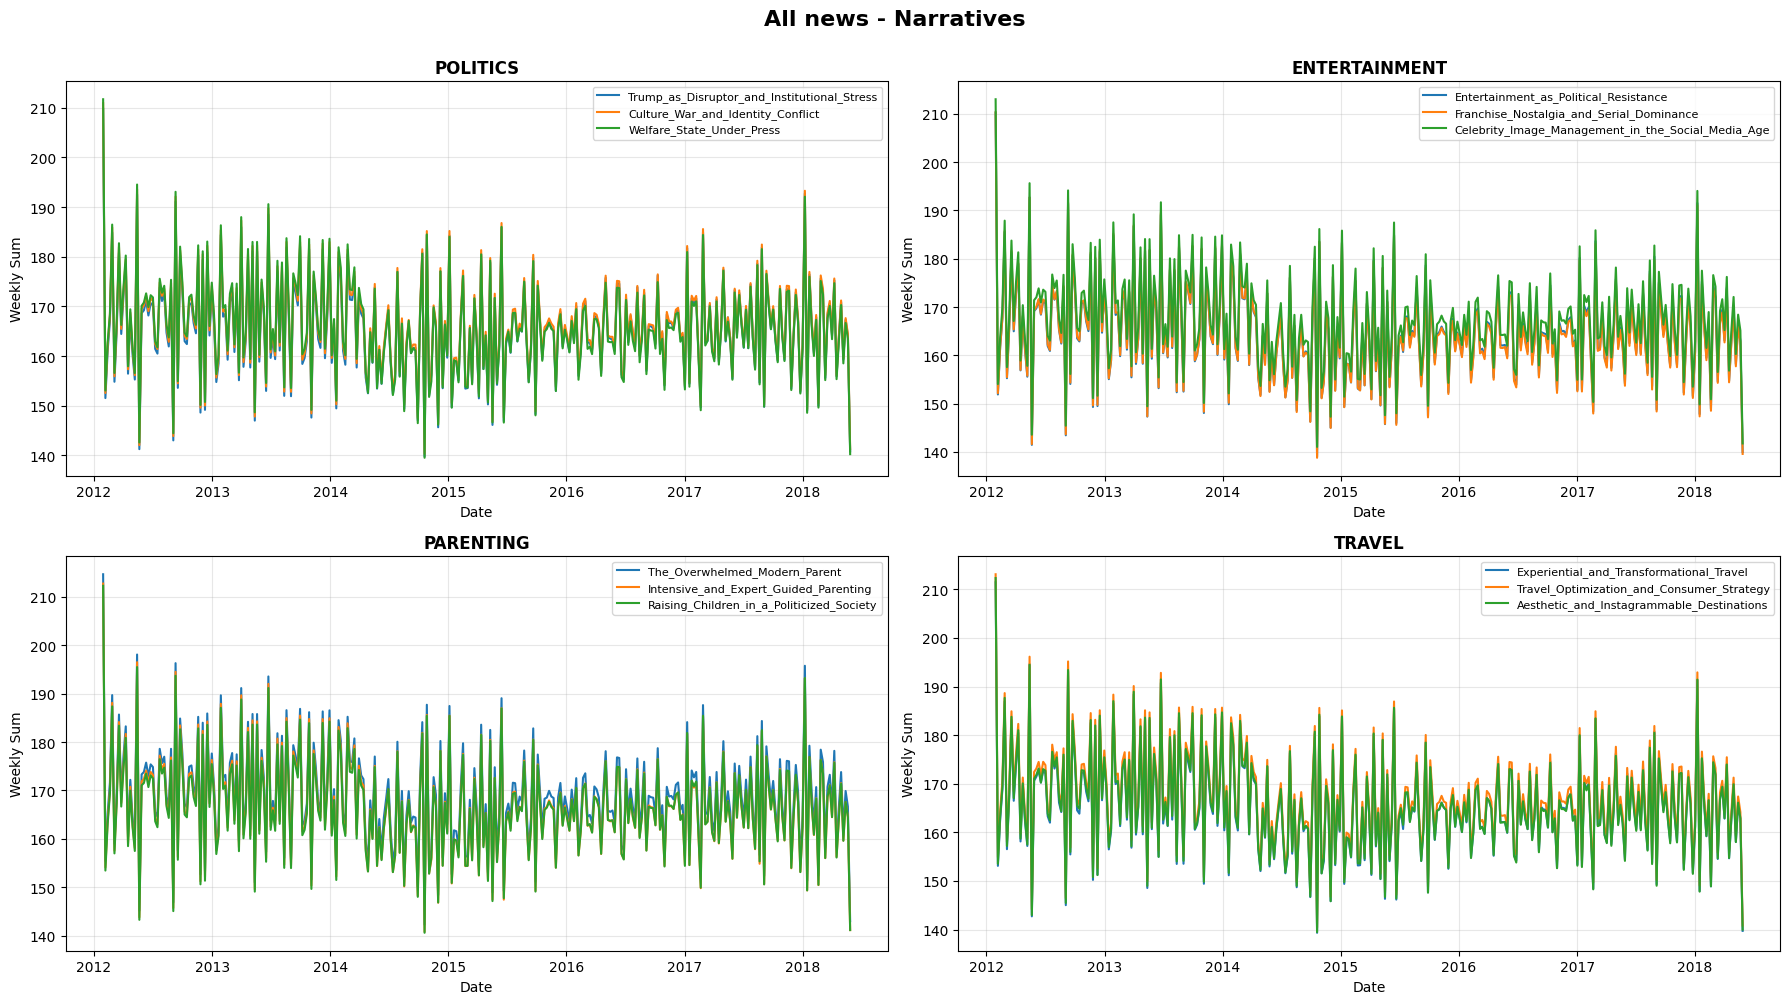
\includegraphics[width=0.85\linewidth]{output_orignal_narratives.png}
    \caption{Weekly cosine similarity between article embeddings and raw narrative vectors $N_i$. 
All time series evolve nearly synchronously, reflecting shared semantic content rather than 
narrative-specific dynamics.}
    \label{fig:output_original}
\end{figure}

\textcolor{ForestGreen}{\bf [CAL: prendre les moyennes et pas les sommes pour être compatibles avec les formules]}

\paragraph{Orthogonalized estimator.}
Applying the estimator of equality~\eqref{eq:estimator} yields clearly differentiated dynamics
(cf. Figure \ref{fig:output_orth}). 

\begin{figure}[hbt!]
    \centering
    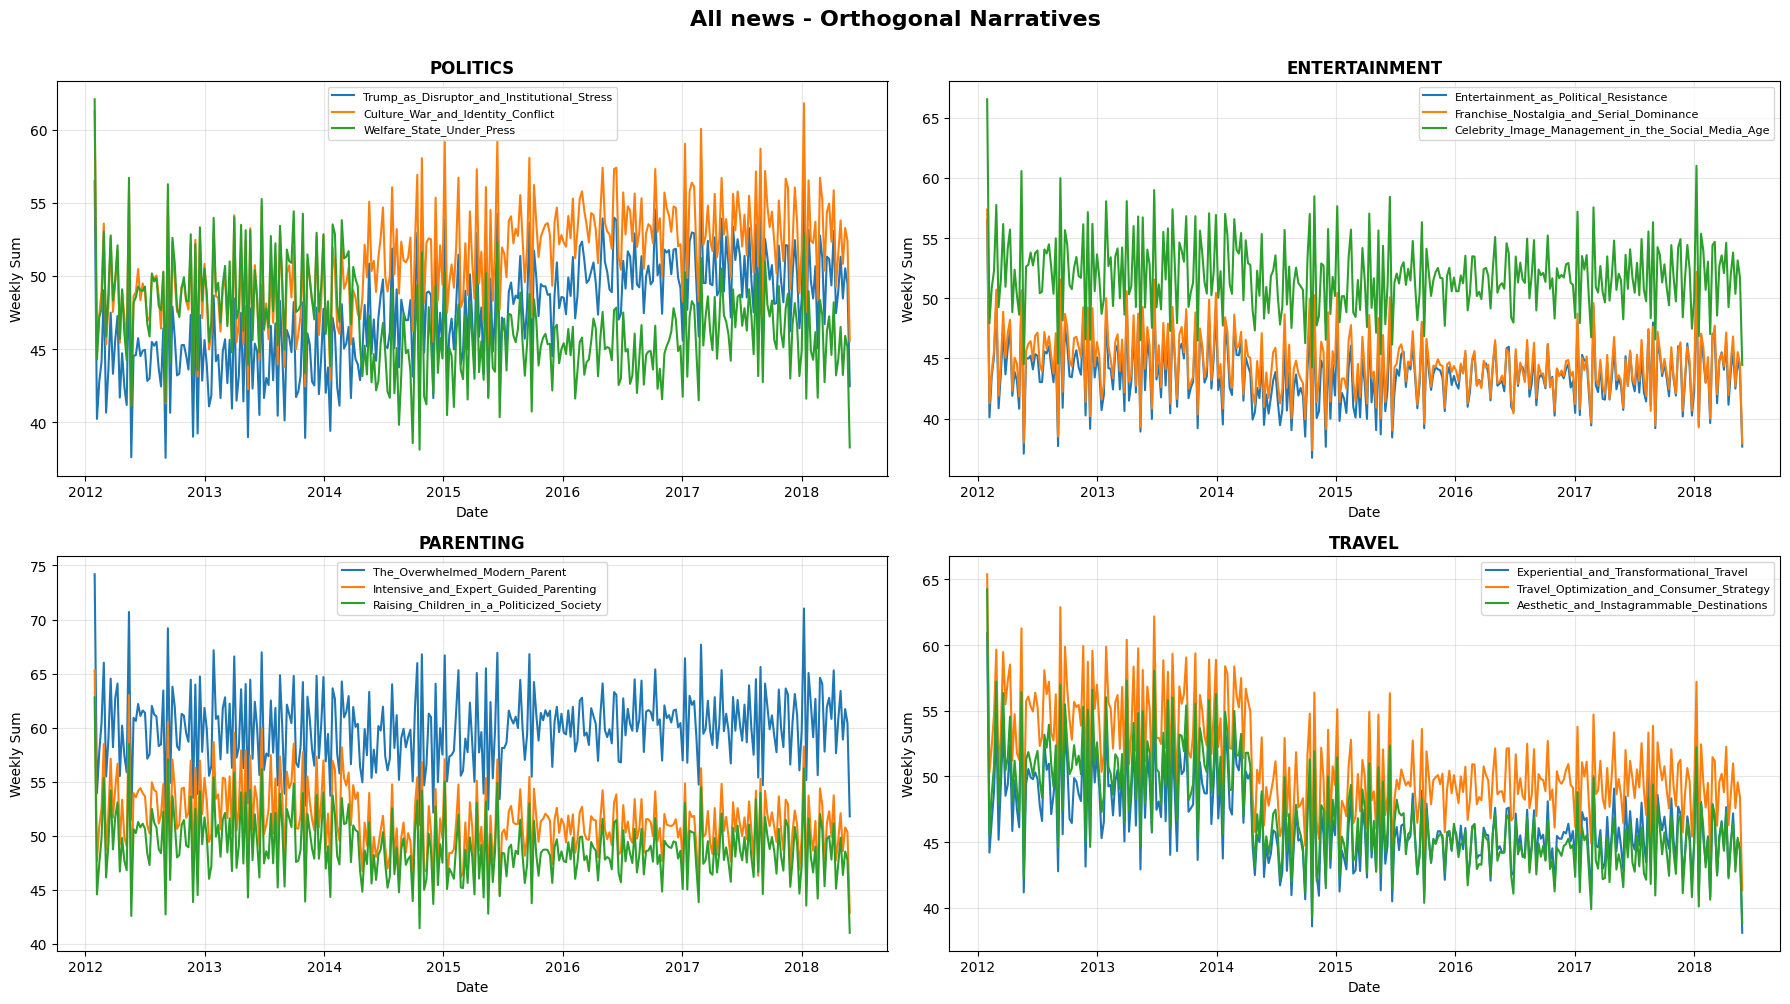
\includegraphics[width=0.85\linewidth]{output_narratives_orth.png}
    \caption{Weekly cosine similarity between article embeddings and orthogonal narrative vectors $V_i$. We can now observe differentiated dynamics}
    \label{fig:output_orth}
\end{figure}

Several features of interest emerge:
\begin{itemize}
    \item The prevalence of \textit{Trump as Disruptor and Institutional Stress}
          rises markedly from 2015-2016 onward, in line with the U.S.\ presidential
          campaign and election.
    \item Concurrently, \textit{Culture War and Identity Conflict} co-increases,
          a genuine co-movement rather than an artefact, since the orthogonalization
          has already removed all shared lexical components.
          A reasonable interpretation may be to consider that it reflects the historical intertwining of immigration, identity, and
          cultural war debates during the Trump campaign.
    \item \textit{Welfare State Under Press} declines relatively over 2016--2017,
          the can be interpreted as welfare policy being displaced by identity politics in
          media coverage.
    \item Travel narratives decline sharply after 2014, matching the structural
          drop in TRAVEL-labelled articles in the dataset.
\end{itemize}

\begin{table}[ht]
\centering
\small
\begin{tabular}{llccc}
\toprule
\textbf{Chapter} & \textbf{Narrative} & $\Delta N_{i,k}$ & $\Delta V_{i,k}$ & $\Delta V_{i,k} - \Delta N_{i,k} $ \\
\midrule

Entertainment &
Beyonce Lemonade and Black Female Artistry &
-0.0008 & 0.0261 & 0.0269 \\
&
The Force Awakens and the Franchise Economy &
0.0037 & 0.0379 & 0.0342 \\
&
Weinstein MeToo and Hollywood Reckoning &
-0.0035 & 0.0140 & 0.0175 \\
&
\emph{Mean chapter} &
-0.0002 & 0.0260 & 0.0262 \\
\addlinespace

Parenting &
Family Separation Crisis and Immigrant Children &
0.0180 & 0.0296 & 0.0116 \\
&
Sandy Hook and the Politics of Child Safety &
0.0155 & 0.0128 & -0.0026 \\
&
Screen Time Panic and the Smartphone Child &
0.0225 & 0.0458 & 0.0233 \\
&
\emph{Mean chapter} &
0.0187 & 0.0294 & 0.0107 \\
\addlinespace

Politics &
ACA Repeal Failure and the Healthcare Battlefield &
0.0089 & 0.0364 & 0.0276 \\
&
Charlottesville and the Mainstreaming of White... &
0.0063 & 0.0259 & 0.0196 \\
&
Trump Election Shock and Democratic Crisis &
0.0143 & 0.0271 & 0.0128 \\
&
\emph{Mean chapter} &
0.0098 & 0.0298 & 0.0200 \\
\addlinespace

Travel &
Airbnb and the Disruption of Travel Infrastructure &
0.0118 & 0.0336 & 0.0219 \\
&
Instagram Travel and the Overtourism Backlash &
0.0115 & 0.0304 & 0.0190 \\
&
Refugee Crisis and the Closing of Borders &
0.0029 & 0.0031 & 0.0002 \\
&
\emph{Mean chapter} &
0.0087 & 0.0224 & 0.0137 \\

\bottomrule
\end{tabular}
\caption{Differences in narrative specificity ($\Delta N_i$), vocabulary richness ($\Delta V_i$), and the resulting gain ($\Delta_{\text{gain}}$) across narratives and chapters.}
\label{tab:delta_summary}
\end{table}

\begin{table}[h!]
\centering
\small
\setlength{\tabcolsep}{4pt}
\begin{tabular}{lcccccccccccc}
\toprule
 & N1 & N2 & N3 & N4 & N5 & N6 & N7 & N8 & N9 & N10 & N11 & N12 \\
\midrule
N1  & 74.828 & 73.820 & 73.768 & 74.743 & 74.612 & 75.546 & 74.386 & 74.061 & 74.242 & 74.191 & 74.109 & 74.759 \\
N2  & 73.820 & 72.827 & 72.775 & 73.737 & 73.608 & 74.529 & 73.384 & 73.064 & 73.243 & 73.192 & 73.111 & 73.753 \\
N3  & 73.768 & 72.775 & 72.723 & 73.685 & 73.556 & 74.476 & 73.332 & 73.012 & 73.191 & 73.140 & 73.060 & 73.701 \\
N4  & 74.743 & 73.737 & 73.685 & 74.660 & 74.529 & 75.461 & 74.302 & 73.977 & 74.159 & 74.108 & 74.026 & 74.676 \\
N5  & 74.612 & 73.608 & 73.556 & 74.529 & 74.398 & 75.329 & 74.172 & 73.848 & 74.028 & 73.977 & 73.896 & 74.544 \\
N6  & 75.546 & 74.529 & 74.476 & 75.461 & 75.329 & 76.271 & 75.099 & 74.772 & 74.954 & 74.903 & 74.820 & 75.476 \\
N7  & 74.386 & 73.384 & 73.332 & 74.302 & 74.172 & 75.099 & 73.947 & 73.625 & 73.803 & 73.751 & 73.670 & 74.316 \\
N8  & 74.061 & 73.064 & 73.012 & 73.977 & 73.848 & 74.772 & 73.625 & 73.305 & 73.481 & 73.429 & 73.348 & 73.992 \\
N9  & 74.242 & 73.243 & 73.191 & 74.159 & 74.028 & 74.954 & 73.803 & 73.481 & 73.661 & 73.610 & 73.529 & 74.174 \\
N10 & 74.191 & 73.192 & 73.140 & 74.108 & 73.977 & 74.903 & 73.751 & 73.429 & 73.610 & 73.561 & 73.479 & 74.124 \\
N11 & 74.109 & 73.111 & 73.060 & 74.026 & 73.896 & 74.820 & 73.670 & 73.348 & 73.529 & 73.479 & 73.398 & 74.042 \\
N12 & 74.759 & 73.753 & 73.701 & 74.676 & 74.544 & 75.476 & 74.316 & 73.992 & 74.174 & 74.124 & 74.042 & 74.692 \\
\bottomrule
\end{tabular}
\caption{Pairwise average similarity scores between the twelve narratives.}
\label{tab:narrative_similarity}
\end{table}

\begin{table}[ht]
\centering
\small
\setlength{\tabcolsep}{4pt}
\begin{tabular}{lcccccccccccc}
\toprule
 & V1 & V2 & V3 & V4 & V5 & V6 & V7 & V8 & V9 & V10 & V11 & V12 \\
\midrule
V1  & 7.211 & 6.071 & 6.187 & 7.145 & 6.796 & 8.343 & 7.115 & 6.584 & 6.495 & 6.555 & 6.482 & 7.113 \\
V2  & 6.071 & 5.112 & 5.209 & 6.016 & 5.721 & 7.024 & 5.989 & 5.542 & 5.469 & 5.520 & 5.458 & 5.990 \\
V3  & 6.187 & 5.209 & 5.310 & 6.131 & 5.831 & 7.158 & 6.102 & 5.646 & 5.574 & 5.627 & 5.563 & 6.105 \\
V4  & 7.145 & 6.016 & 6.131 & 7.083 & 6.735 & 8.266 & 7.045 & 6.518 & 6.439 & 6.500 & 6.426 & 7.053 \\
V5  & 6.796 & 5.721 & 5.831 & 6.735 & 6.405 & 7.862 & 6.703 & 6.202 & 6.122 & 6.180 & 6.110 & 6.706 \\
V6  & 8.343 & 7.024 & 7.158 & 8.266 & 7.862 & 9.656 & 8.237 & 7.623 & 7.513 & 7.579 & 7.497 & 8.227 \\
V7  & 7.115 & 5.989 & 6.102 & 7.045 & 6.703 & 8.237 & 7.038 & 6.516 & 6.400 & 6.451 & 6.385 & 7.004 \\
V8  & 6.584 & 5.542 & 5.646 & 6.518 & 6.202 & 7.623 & 6.516 & 6.035 & 5.921 & 5.965 & 5.906 & 6.479 \\
V9  & 6.495 & 5.469 & 5.574 & 6.439 & 6.122 & 7.513 & 6.400 & 5.921 & 5.857 & 5.913 & 5.845 & 6.415 \\
V10 & 6.555 & 5.520 & 5.627 & 6.500 & 6.180 & 7.579 & 6.451 & 5.965 & 5.913 & 5.978 & 5.903 & 6.481 \\
V11 & 6.482 & 5.458 & 5.563 & 6.426 & 6.110 & 7.497 & 6.385 & 5.906 & 5.845 & 5.903 & 5.834 & 6.404 \\
V12 & 7.113 & 5.990 & 6.105 & 7.053 & 6.706 & 8.227 & 7.004 & 6.479 & 6.415 & 6.481 & 6.404 & 7.030 \\
\bottomrule
\end{tabular}
\caption{Pairwise average overlap scores between the twelve vocabulary representations. Vocabulary identifiers (V1--V12) are defined in Table~\ref{tab:vocabulary_ids}.}
\label{tab:vocabulary_overlap}
\end{table}

\begin{table}[ht!]
\centering
\small
\begin{tabular}{ll}
\toprule
ID & Narrative \\
\midrule
N1  & Entertainment: Celebrity Image Management in the Social Media Age \\
N2  & Entertainment: Entertainment as Political Resistance \\
N3  & Entertainment: Franchise Nostalgia and Serial Dominance \\
N4  & Parenting: Intensive and Expert-Guided Parenting \\
N5  & Parenting: Raising Children in a Politicized Society \\
N6  & Parenting: The Overwhelmed Modern Parent \\
N7  & Politics: Culture War and Identity Conflict \\
N8  & Politics: Trump as Disruptor and Institutional Stress \\
N9  & Politics: Welfare State Under Pressure \\
N10 & Travel: Aesthetic and Instagrammable Destinations \\
N11 & Travel: Experiential and Transformational Travel \\
N12 & Travel: Travel Optimization and Consumer Strategy \\
\bottomrule
\end{tabular}
\caption{Mapping between narrative identifiers and narrative names.}
\label{tab:narrative_ids}
\end{table}



% -------------------------------------------------------
\section{A Generative Model and Its Statistical Properties}
\label{sec:model}
% -------------------------------------------------------
{\color{red}[CAL] je fais ça pour introduire cette section qui devrait être positionnée juste après l'intro.}

In this section we explain the model for the structure of narrative in the embedding space that supports our approach.
Qualitatively, we assume that any text $X_n$ of our corpus (typically, in our case, News) combines an exposure to our narratives of interest $(V_i)_{1\leq i\leq K}$ plus exposures to generic English context and narratives that are not of interest for us.
We consider that our narratives are \emph{pure} in the sense that they are orthogonal in the embedding space: to get back to the example in the introduction that is ``D. Trump will win the election'' vs. ``H. Clinton will win the election'', we consider that they are at least three pure narratives in play: {\tt winner=Trump}, {\tt winner=Clinton}, {\tt elections}. They are probably others hidden in the English wording used to express the narratives.
But we consider taking $V_1$ (respectively $V_2$ and $V_3$) as the best representative of {\tt winner=Trump} (resp. {\tt winner=Clinton} and {\tt elections}) \emph{such that they are orthogonal two by two and that their norm is one}, is a proper choice of temporal monitoring of narrative dominance in the database $(t_n,X_n)_{1\leq n\leq N}$.

\begin{definition}[Collection of pure narratives]
Any collection $V_1,\ldots,V_K$ of narrative embedded in $\calH \subset \R^d$ that are orthogonal two by two and of norm one is a collection of \emph{pure narratives}.
\end{definition}

We are not claiming it is possible to generate three English sentences describing these three pure narratives, but we provide in Section \ref{sec:ortho} a methodology to deduce pure narrative candidate vectors from any list of texts which narratives are not pure. The question of generating English texts rendering a pure narrative is out of the scope of this paper, because, as it is exposed in this section, it is not needed to monitor the prevalence of narratives in texts.

\subsection{The Statement of Our Generative Model}
\label{sec:model:generative_model}

{\color{red}
At this stage of our reasoning, consider we have access to a collection of pure narratives. As a consequence we can express $X(\omega)$ the embedding of an occurrence $\omega$ of a text (typically a News article)  
%Let $\mathcal{H} \cong \R^d$ denote the embedding space.
%We model the corpus as a collection of article embeddings
%any News articles of our collection
%$\{X_n\}_{n=1}^N$ %can be 
%where each $X_n \in \mathcal{H}$ follows the generative model:
as $X(\omega) = \sum_{i=1}^{K} \alpha_{i}(\omega)\, V_i + \varepsilon(\omega)$
where $\alpha_{i}(\omega)$ is a binary narrative presence indicators, and $\varepsilon(\omega)$ lies in the orthogonal of the subspace spanned by $(V_1,\ldots,V_K)$. It thus contains references to a lot of concepts that have nothing to do with our pure narratives.

This framework is supported by a probability space generated by the law of $(\alpha_1,\ldots,\alpha_K,\varepsilon)$, indeed by a filtration $(\calF_t)_t$ as soon as we add time via $\tau(\omega)$ the day (and time) of the occurrence of this text.

For simplicity, we will take the $\alpha_i$ independent and identically distributed as a Bernoulli, with a parameter $p_{i,t}$ that is adapted to $\calF_t$. It means that at each time $t$ the expected presence of the pure narrative $V_i$ in an article is $\Esp(\alpha_i|\calF_t)=p_{i,t}$.
For simplicity again, we will take $\varepsilon\sim\calN(0,\sigma_\varepsilon)$ distributed like a Gaussian: from the viewpoint of our analysis it behaves like a centered noise, orthogonal (i.e. independent) to any $\alpha_i$.

\begin{center}
    \color{ForestGreen} On peut maintenant écrire la formule (\ref{eq:esp:scalar}) et ses amies très simplement. Que l'on retrouvera plus tard sur la base de données: les conditionnement par $t_n$ sont en fait des conditionnement par $\calF_t$ (dès que $\tau(\omega)$ est un temps d'arrêt).
    \\
    Ensuite on dit juste:
\end{center}

For notational convenience we will shortcut the heavy writing of $\omega$ and simply refer to a database $(t_n,X_n)_n$ that is the collection of observations.
The natural notation is then:
\begin{equation}
    \label{eq:generative}
    X_n = \sum_{i=1}^{K} \alpha_{i,n} V_i + \varepsilon_n.
\end{equation}
where ...}
% \begin{itemize}
%     \item $t_n \in \{1,\ldots,T\}$ denotes the publication date of article $n$;
%     \item $\alpha_n^i \overset{\mathrm{i.i.d.}}{\sim} \mathcal{B}(p_i(t_n))$ are
%           binary narrative presence indicators: a narrative is either present or
%           absent in a given article;
%     \item $\varepsilon_n \in \mathcal{V}^\perp :=
%           \operatorname{Vect}(V_1,\ldots,V_K)^\perp$
%           captures content unrelated to any of the $K$ narratives
%           (author style, secondary facts, unmodeled topics), with
%           $\E[\varepsilon_n] = 0$;
%     \item the articles $(X_n)_{n=1}^N$ are \emph{independent} by construction,
%           as the $\alpha_n^i$ are i.i.d.\ across articles and the noise terms
%           $\varepsilon_n$ are independent.
% \end{itemize}
\textcolor{ForestGreen}{[CAL] pas de panique j'ai juste commenté l'ancien texte.}

\paragraph{Narrative sparsity hypothesis.}\textcolor{red}{[CAL] on peut s'en passer car maintenant c'est vrai \emph{par construction}.}
The binary assumption on $\alpha_n^i$ is qualitatively justified:
a news article typically covers a small number of distinct narratives,
each either explicitly present or absent.
The continuous intensity variation observed at the aggregate level
arises from the \emph{frequency} with which each narrative appears
across the corpus, not from a continuous activation at the article level.

\paragraph{Orthogonal decomposition.}\textcolor{red}{[CAL] je pense qu'on a à peine à la dire maintenant (cette décomposition sera expliquée/justifiée par Stiefel)?}
Since $\{V_i\}_{i=1}^K$ are orthonormal, they span a subspace
$\mathcal{V} = \operatorname{Vect}(V_1,\ldots,V_K)$,
and $\mathcal{H} = \mathcal{V} \oplus \mathcal{V}^\perp$.
Any $X_n$ admits a unique decomposition $X_n = X_n^\parallel + X_n^\perp$,
where $X_n^\parallel \in \mathcal{V}$ corresponds to the sum of active narratives
and $X_n^\perp = \varepsilon_n$.

% -------------------------------------------------------
\subsection{Time Discretization and Prevalence}
\label{sec:model:prevalence}
% -------------------------------------------------------
\textcolor{red}{[CAL] Cette sous-section est bien: il faut juste la présenter comme un conditionnement par des temps d'arrêts de formules plus probabilistes qu'il faudra écrire au dessus. Ce n'est pas vraiment \emph{Time Discretization}, c'est \emph{Temporal Conditioning}...}


Time is discretized into periods indexed by $t \in \{1,\ldots,T\}$,
without fixing \emph{a priori} the granularity of the discretization
(day, week, month, etc.). For each period $t$, we denote by:
\begin{equation}
    \mathcal{C}_t := \{n : t_n = t\}, \qquad n_t := |\mathcal{C}_t|
\end{equation}
the set and number of articles published during period $t$.

\paragraph{Conditional prevalence.}
The prevalence of narrative $i$ at time $t$ is defined as the probability
that a given article published at time $t$ carries narrative $i$:
\begin{equation}
    \label{eq:prevalence}
    p_i(t) := \E\bigl[V_i^\top X_n \mid t_n = t\bigr].
\end{equation}

We show that this definition coincides with the one given in the generative model by using the orthonormality of the $V_i$ and $\varepsilon_n \in \operatorname{Vect}(V_1,\ldots,V_K)^\perp$:
\begin{equation}\label{eq:esp:scalar}
    \E\bigl[V_i^\top X_n \mid t_n = t\bigr]
    = \sum_{k=1}^K \E\bigl[\alpha_n^k \mid t_n = t\bigr]V_i^\top V_k
      + \E\bigl[V_i^\top \varepsilon_n\bigr]
    = \sum_{k=1}^K p_k(t)\underbrace{V_i^\top V_k}_{=\,\delta_{ik}}
      + \E\bigl[\underbrace{V_i^\top \varepsilon_n]}_{=\,0} \mid t_n = t\bigr]
    = p_i(t).
\end{equation}


\paragraph{Absolute frequency.}
Alternatively, one may define the absolute frequency of narrative $i$ at
time $t$, which jointly captures narrative intensity and publication volume:
\begin{equation}
    \label{eq:abs_freq}
    q_i(t) := \E\bigl[V_i^\top X_n \cdot \mathbf{1}_{t_n = t}\bigr]
\end{equation}


% -------------------------------------------------------
\subsection{Empirical Estimators}
\label{sec:model:estimator}
% -------------------------------------------------------
\textcolor{red}{[CAL] Cette sous-section est super.}


The natural empirical counterparts of $p_i(t)$ and $q_i(t)$ are:
\begin{align}
    \hat{p}_i(t) &= \frac{1}{n_t}\sum_{n \in \mathcal{C}_t} V_i^\top X_n,
    \label{eq:estimator_p}\\
    \hat{q}_i(t) &= \frac{1}{N}\sum_{n \in \mathcal{C}_t} V_i^\top X_n
                  = \frac{n_t}{N}\,\hat{p}_i(t).
    \label{eq:estimator_q}
\end{align}

\paragraph{Unbiasedness of $\hat{p}_i(t)$.}
Conditioning on $\mathcal{C}_t$ and using the fact that knowing $t_n$, $X_n$ is independent of $\mathcal{C}_t$:
\begin{equation}
    \E\bigl[\hat{p}_i(t) \mid \mathcal{C}_t\bigr]
    = \frac{1}{n_t}\sum_{n \in \mathcal{C}_t}
      \E\bigl[V_i^\top X_n \mid t_n = t\bigr]
    = \frac{1}{n_t}\sum_{n \in \mathcal{C}_t} p_i(t)
    = p_i(t),
\end{equation}

By the law of iterated expectations, $\hat{p}_i(t)$ is therefore an
unbiased estimator of $p_i(t)$:
\begin{equation}
    \E\bigl[\hat{p}_i(t)\bigr]
    = \E\Bigl[\E\bigl[\hat{p}_i(t) \mid \mathcal{C}_t\bigr]\Bigr]
    = p_i(t).
\end{equation}

\paragraph{Unbiasedness of $\hat{q}_i(t)$.}
Because $N$ is fixed, we can exchange expectation and summation directly:
\begin{equation}
    \E\bigl[\hat{q}_i(t)\bigr]
    = \frac{1}{N}\sum_{n=1}^N
      \E\bigl[V_i^\top X_n \cdot \mathbf{1}_{t_n = t}\bigr] = q_i(t).
\end{equation}

\JAMM{fin de la tentative}


\textcolor{ForestGreen}{\bf [CAL: on peut introduire $${\hat q}_i(t) = \frac{1}{|\mbox{all}|}
    \sum_{X \in \mathcal{C}_t} V_i^\top X_t$$ qui est un estimateur de $\E\bigl[V_i^\top X{\color{red}\,\wedge\, \mbox{week}=t}\bigr] = q_i(t)$ et expliquer la (non) dépendance au nombre de news de la semaine; c'est d'ailleurs assez logique de prendre le moyenne surtout pour le contrefactuel, car ça ``stationnarise'' par semaine]}

\bigskip

\JAMM{Tentative de réécriture en introduisant les quantités $q_i(t)$ et $p_i(t)$ ci-dessous}


\begin{table}[ht]
\centering
\small
\begin{tabular}{llccc}
\toprule
\textbf{Chapter} & \textbf{Narrative} & $\Delta N_{i,k}$ & $\Delta V_{i,k}$ & $\Delta V_{i,k} - \Delta N_{i,k}$ \\
\midrule

Entertainment &
Celebrity Image Management in the Social Media... &
-0.0085 & 0.0050 & 0.0135 \\
&
Entertainment as Political Resistance &
-0.0063 & 0.0116 & 0.0179 \\
&
Franchise Nostalgia and Serial Dominance &
-0.0019 & 0.0267 & 0.0285 \\
&
\emph{Mean chapter} &
-0.0055 & 0.0144 & 0.0200 \\
\addlinespace

Parenting &
Intensive and Expert Guided Parenting &
0.0256 & 0.0304 & 0.0047 \\
&
Raising Children in a Politicized Society &
0.0216 & 0.0174 & -0.0042 \\
&
The Overwhelmed Modern Parent &
0.0224 & 0.0133 & -0.0092 \\
&
\emph{Mean chapter} &
0.0232 & 0.0203 & -0.0029 \\
\addlinespace

Politics &
Culture War and Identity Conflict &
0.0058 & 0.0294 & 0.0236 \\
&
Trump as Disruptor and Institutional Stress &
0.0073 & 0.0356 & 0.0283 \\
&
Welfare State Under Press &
0.0032 & 0.0190 & 0.0158 \\
&
\emph{Mean chapter} &
0.0054 & 0.0280 & 0.0225 \\
\addlinespace

Travel &
Aesthetic and Instagrammable Destinations &
0.0158 & 0.0334 & 0.0175 \\
&
Experiential and Transformational Travel &
0.0129 & 0.0248 & 0.0118 \\
&
Travel Optimization and Consumer Strategy &
0.0156 & 0.0371 & 0.0215 \\
&
\emph{Mean chapter} &
0.0148 & 0.0317 & 0.0169 \\

\bottomrule
\end{tabular}
\caption{Differences in narrative specificity ($\Delta N_i$), vocabulary richness ($\Delta V_i$), and the resulting gain ($\Delta_{\text{gain}}$) across narratives and chapters.}
\label{tab:delta_summary}
\end{table}